\documentclass[5p]{elsarticle}

\usepackage{lineno,hyperref}
\usepackage{xcolor}
\usepackage{amssymb,amsmath}

\modulolinenumbers[5]

\journal{Astroparticle Physics}

\bibliographystyle{elsarticle-num}%`Elsevier LaTeX' style

\begin{document}

\begin{frontmatter}

\title{The effective nucleon axial mass approach and quasielastic neutrino event rates in NO$\nu$A and Super-Kamiokande}

%% Group authors with affiliations in footnotes:
\author[ITEP,JINR]{K.~Kuzmin}
\ead{kkuzmin@theor.jinr.ru}

\author[JINR]{V.~Naumov}
\ead{vnaumov@theor.jinr.ru}

\author[JINR]{O.~Petrova\corref{correspondingauthor}}
\cortext[correspondingauthor]{Corresponding author}
\ead{redponick@gmail.com}

\author[JINR]{I.~Shandrov}
\ead{ishandrov@yahoo.co.uk}

\address[ITEP]{Institute for Theoretical and Experimental Physics, Bolshaya Cheremushkinskaya 25, RU-117218 Moscow, Russia}
\address[JINR]{Joint Institute for Nuclear Research, Joliot-Curie 6, RU-141980 Dubna, Russia}

\begin{abstract}
For the accurate interpretation of neutrino experiment results, in particular, for the neutrino mixing parameter extraction, it is necessary to study theoretical uncertainty in predicted count rates in detectors.

Quasielastic neutrino-nucleus interaction makes the main contribution to the count rate of so-called muon-like and electron-like events identified as single-ring events fully contained in water-Cherenckov detectors like Super-Kamiokande. Also quasielastic scattering events can be identified separately in tracking detectors, e.g. NO$\nu$A.

An essential source of calculation uncertainty belongs to cross sections of neutrino interactions with nucleons and nuclei. There is currently no generally accepted single nuclear model, applicable in a wide energy range, from threshold to extremely high values. Also there is a problem with nucleon structure functions, especially, with so-called nucleon axial mass, an important phenomenological parameter characterizing the axial-vector and pseudoscalar form factors. The range of quasielastic axial mass values used in the current Monte Carlo neutrino generators for a number of experiments (from 0.99 GeV in T2K to 1.2 GeV in Super-Kamiokande) seems to be unreasonably wide and distorting the interpretation of the experimental results.

Phenomenological solution for both these problems is to apply the effective axial mass, which means the use of the relativistic Fermi gas model of the nucleus at the same time with the introduction of the axial form factor parameterization. From the statistical analysis of available accelerator data on quasielastic neutrino scattering we extract the shape of the parameterization and optimal values of the parameters, which can be recommended for use in the neutrino generators.

\textbf{Brief alternative version}

In this study, we estimate the error in quasielastic event rate predictions for atmospheric and accelerator neutrino experiments caused by the uncertainty in the nucleon axial mass value. It follows from our analysis that the impact of the axial mass uncertainty is comparable in magnitude with the expected neutrino oscillation effect itself. We propose a simple phenomenological method which allows to describe experimental quasielastic neutrino interaction data consistently and decrease uncertainty in the extracted neutrino mixing parameters.

\end{abstract}

\begin{keyword}
neutrino oscillation\sep quasielastic cross section\sep nucleon axial mass\sep Super-Kamiokande
\end{keyword}

\end{frontmatter}

\linenumbers

\section{Introduction: The axial mass problem}
The axial-vector and pseudoscalar form-factors in the electroweak nucleon current are the subject of long-standing theoretical and experimental efforts. However, these values still remain rather poorly known. Within the framework of the conventional parametrizations, both form-factors are characterized by a single phenomenological parameter, nucleon axial mass $M_{A}$:
\begin{equation}
F_{P}(Q^{2})={}\frac{2M^{2}}{m_{\pi}^{2}+Q^{2}}F_{A}(Q^{2}),\\
F_{A}(Q^{2})={}g_{A}\left(1+\frac{Q^{2}}{M_{A}^{2}}\right)^{-2},
\label{formfactors}
\end{equation}
here $g_{A}=-1.2695$ --- axial-vector coupling, $m_{\pi}$ --- charged pion mass, $M=(M_{n}+M_{p})/2$ --- isoscalar nucleon mass, $Q^{2}=-q^{2}$, where $q^{2}$ --- squared 4-momentum transfer~\cite{Kuzmin:2007kr}.

Global statistical analysis of all available and mutually consistent data on the total and differential cross sections for the $\nu_{\mu}$ and $\bar\nu_{\mu}$ quasielastic scattering (QES) on hydrogen and deuterium and also on different nuclear targets at high energies us to extract the best-fit value of nucleon axial mass: $M_{A}=1.012\pm0.031$\,GeV~\cite{Kuzmin:2014}. In Fig.~\ref{TotalCS} we demonstrate several examples of this analysis. The problem is in huge disagreement between the obtained best-fit value and the value extracted in the K2K and (especially) MiniBooNE experiments. Figures~\ref{K2K} and \ref{MiniBooNE} represent the K2K and the MiniBooNE measurements: $M_{A}=1.20\pm0.12$\,GeV~\cite{Gran:2006jn} and $M_{A}=1.35\pm0.17$\,GeV~\cite{AguilarArevalo:2010zc}, respectively. Thus, there is no consensus about right value of nucleon axial mass.

\begin{figure}[htb!]
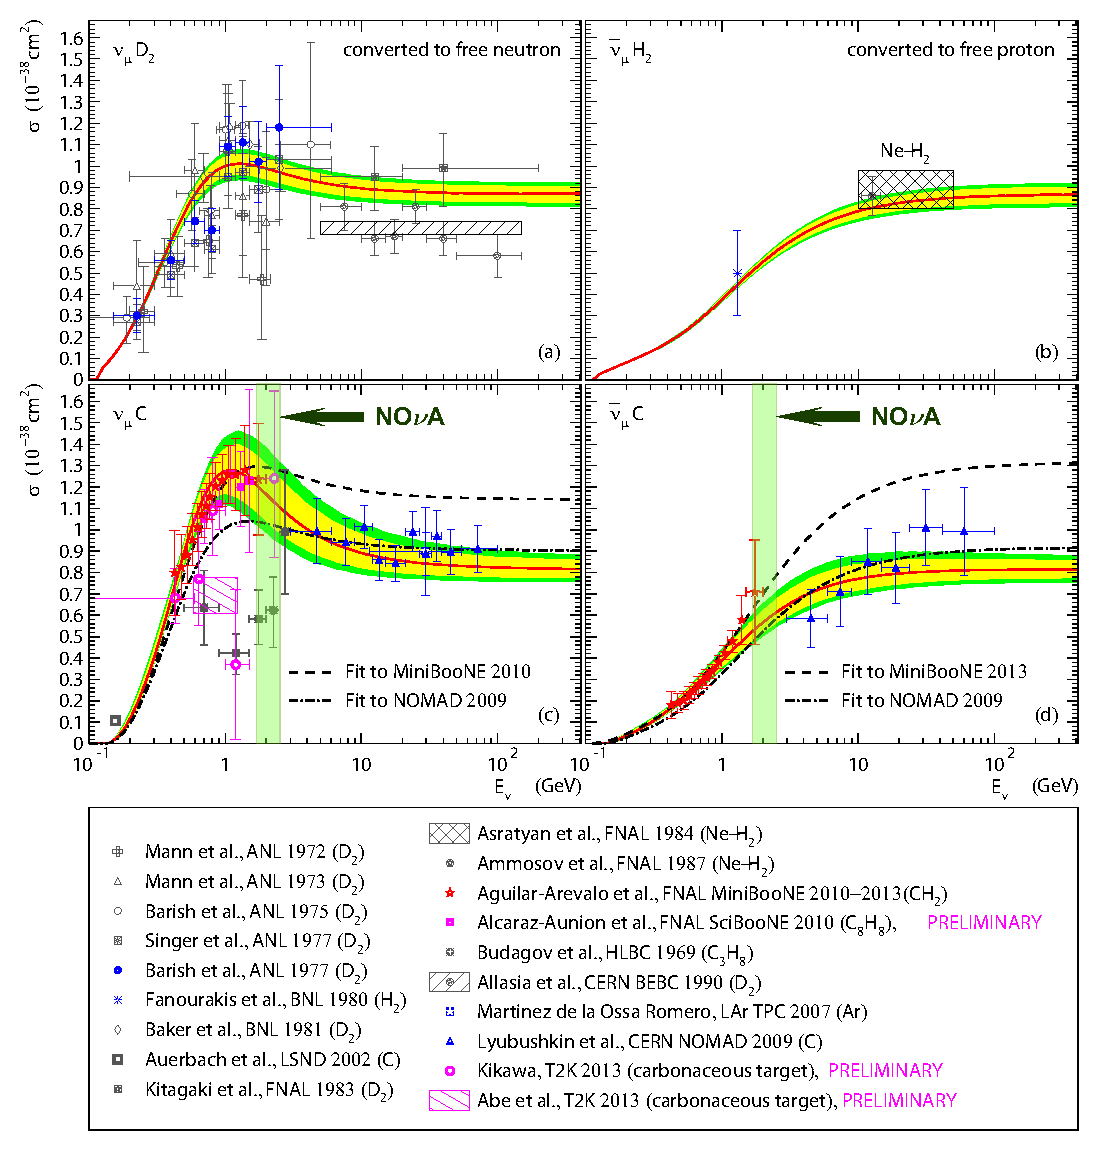
\includegraphics[width=0.5\textwidth]{./QES/sQESCC_101.2.31.301.1b_2_BBBA25_NT_1_NOvA.eps}
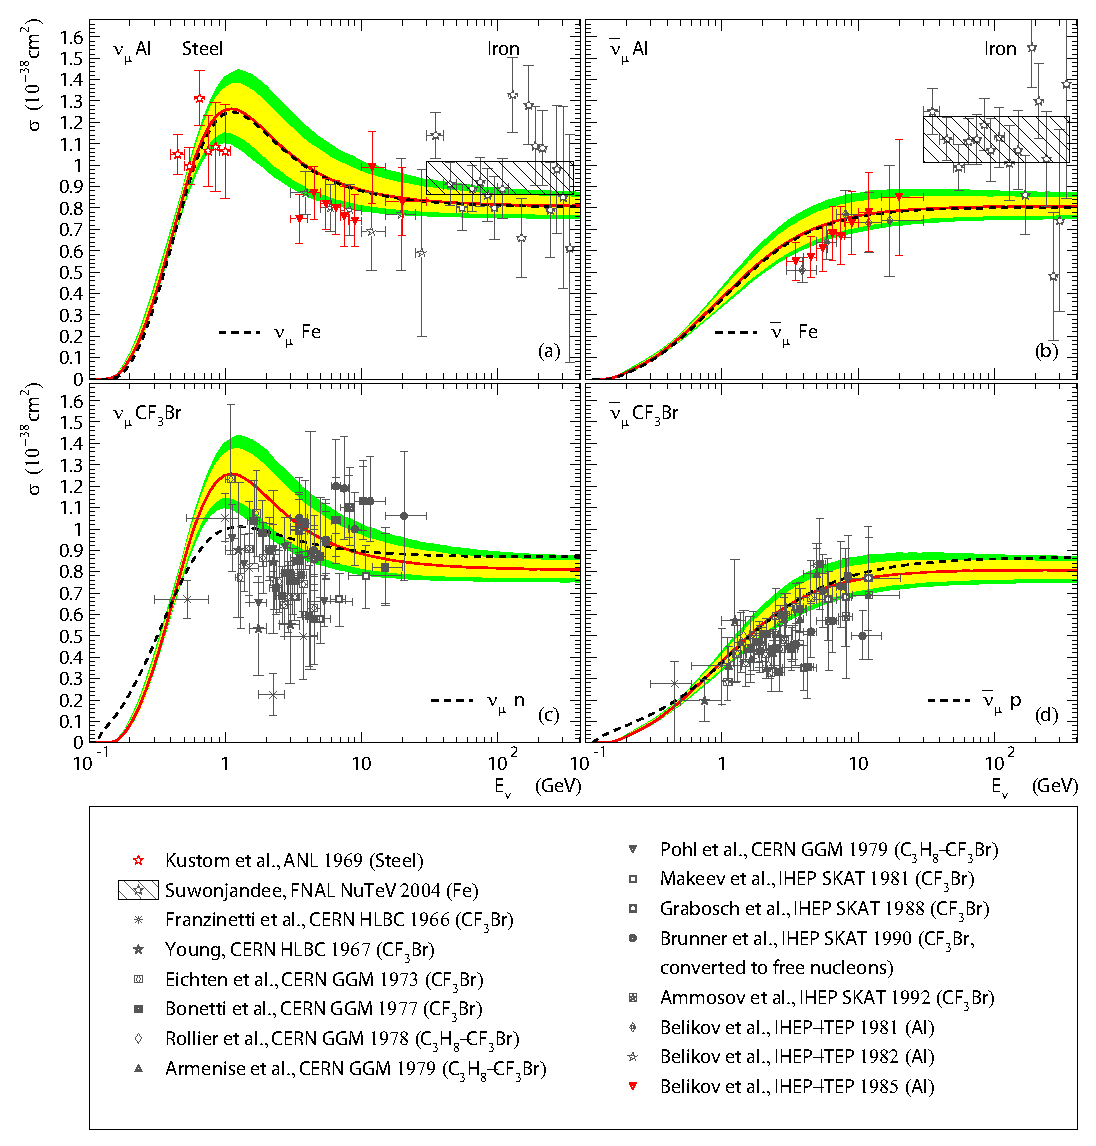
\includegraphics[width=0.5\textwidth]{./QES/sQESCC_101.2.31.301.1b_2_BBBA25_NT_2.eps}
\caption{\label{TotalCS}\textbf{Total QES $\nu_{\mu}n$ \& $\bar\nu_{\mu}p$ cross sections} measured in experiments with deuterium, hydrogen and other targets. The light points are excluded from the global fit being either superseded by newer experiments, or not satisfying our selection criteria (see Ref.\cite{Kuzmin:2007kr} for more details and for the full set of the experimental data). The dash-dotted curves show cross sections calculated with the NOMAD result: $M_A=1.05\pm0.02\pm0.06$\,GeV~\cite{Lyubushkin:2008pe}. The \textbf{dashed curves correspond} the MiniBooNE result: $M_{A}=1.35\pm0.17$\,GeV~\cite{AguilarArevalo:2010zc}. The solid curve represent the effective axial mass application. The widths of the inner (outer) bands correspond to the $1\sigma$ ($2\sigma$) standard deviations from the fit caused by the uncertainties in determination of $M_{A}$ including the spectrum normalizations}
\end{figure}

\begin{figure}[htb!]
\begin{center}
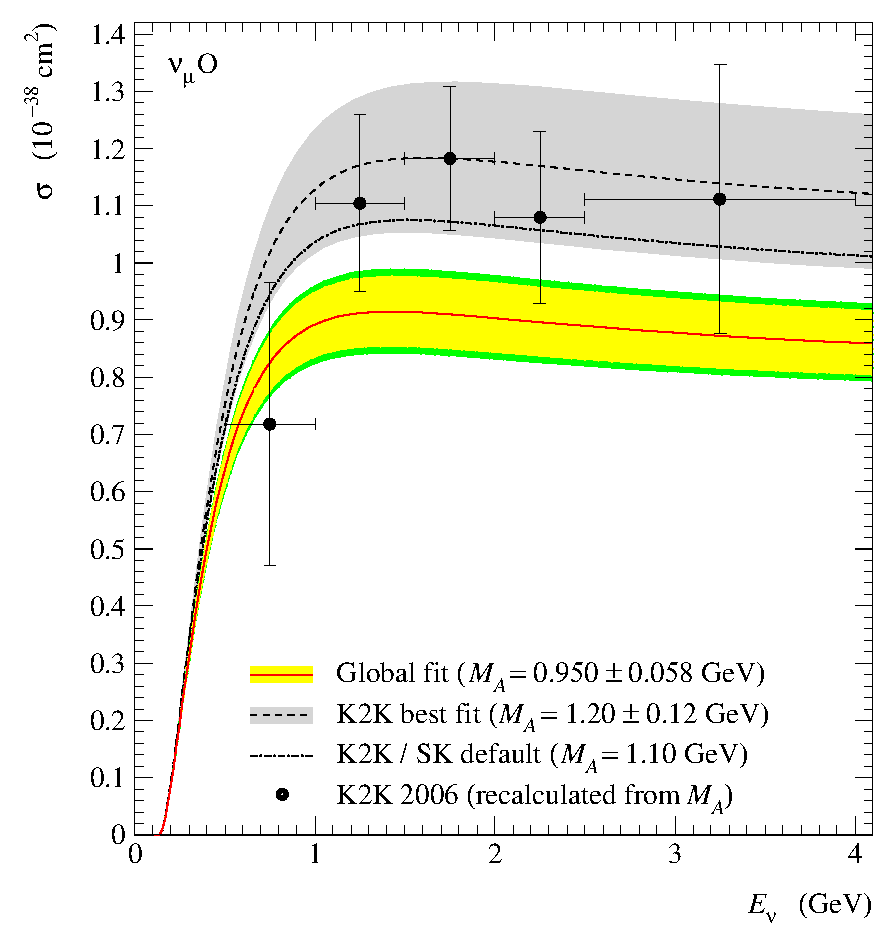
\includegraphics[width=0.45\textwidth]{./QES/sQESCC_K2K06_101.3.00.301.00_2_BBBA25_SM.eps}
\caption{\label{K2K}\textbf{A comparison of the QES $\nu_{\mu}$ cross sections} per neutron bound in oxygen evaluated with different values of $M_{A}$. The dashed curve with accompanying band corresponds to the K2K extraction of $M_{A}$~\cite{Gran:2006jn}. The dash-dotted curve is the cross section calculated with $M_{A}=1.1$\,GeV, the value which was the K2K and SK\,I default before 2006~\cite{Gran:2006jn,Ashie:2005ik}. The points in Fig.~\ref{K2K} represent the total QES cross section reconstructed from the ``raw'' K2K data}
\end{center}
\end{figure}

\begin{figure}[htb!]
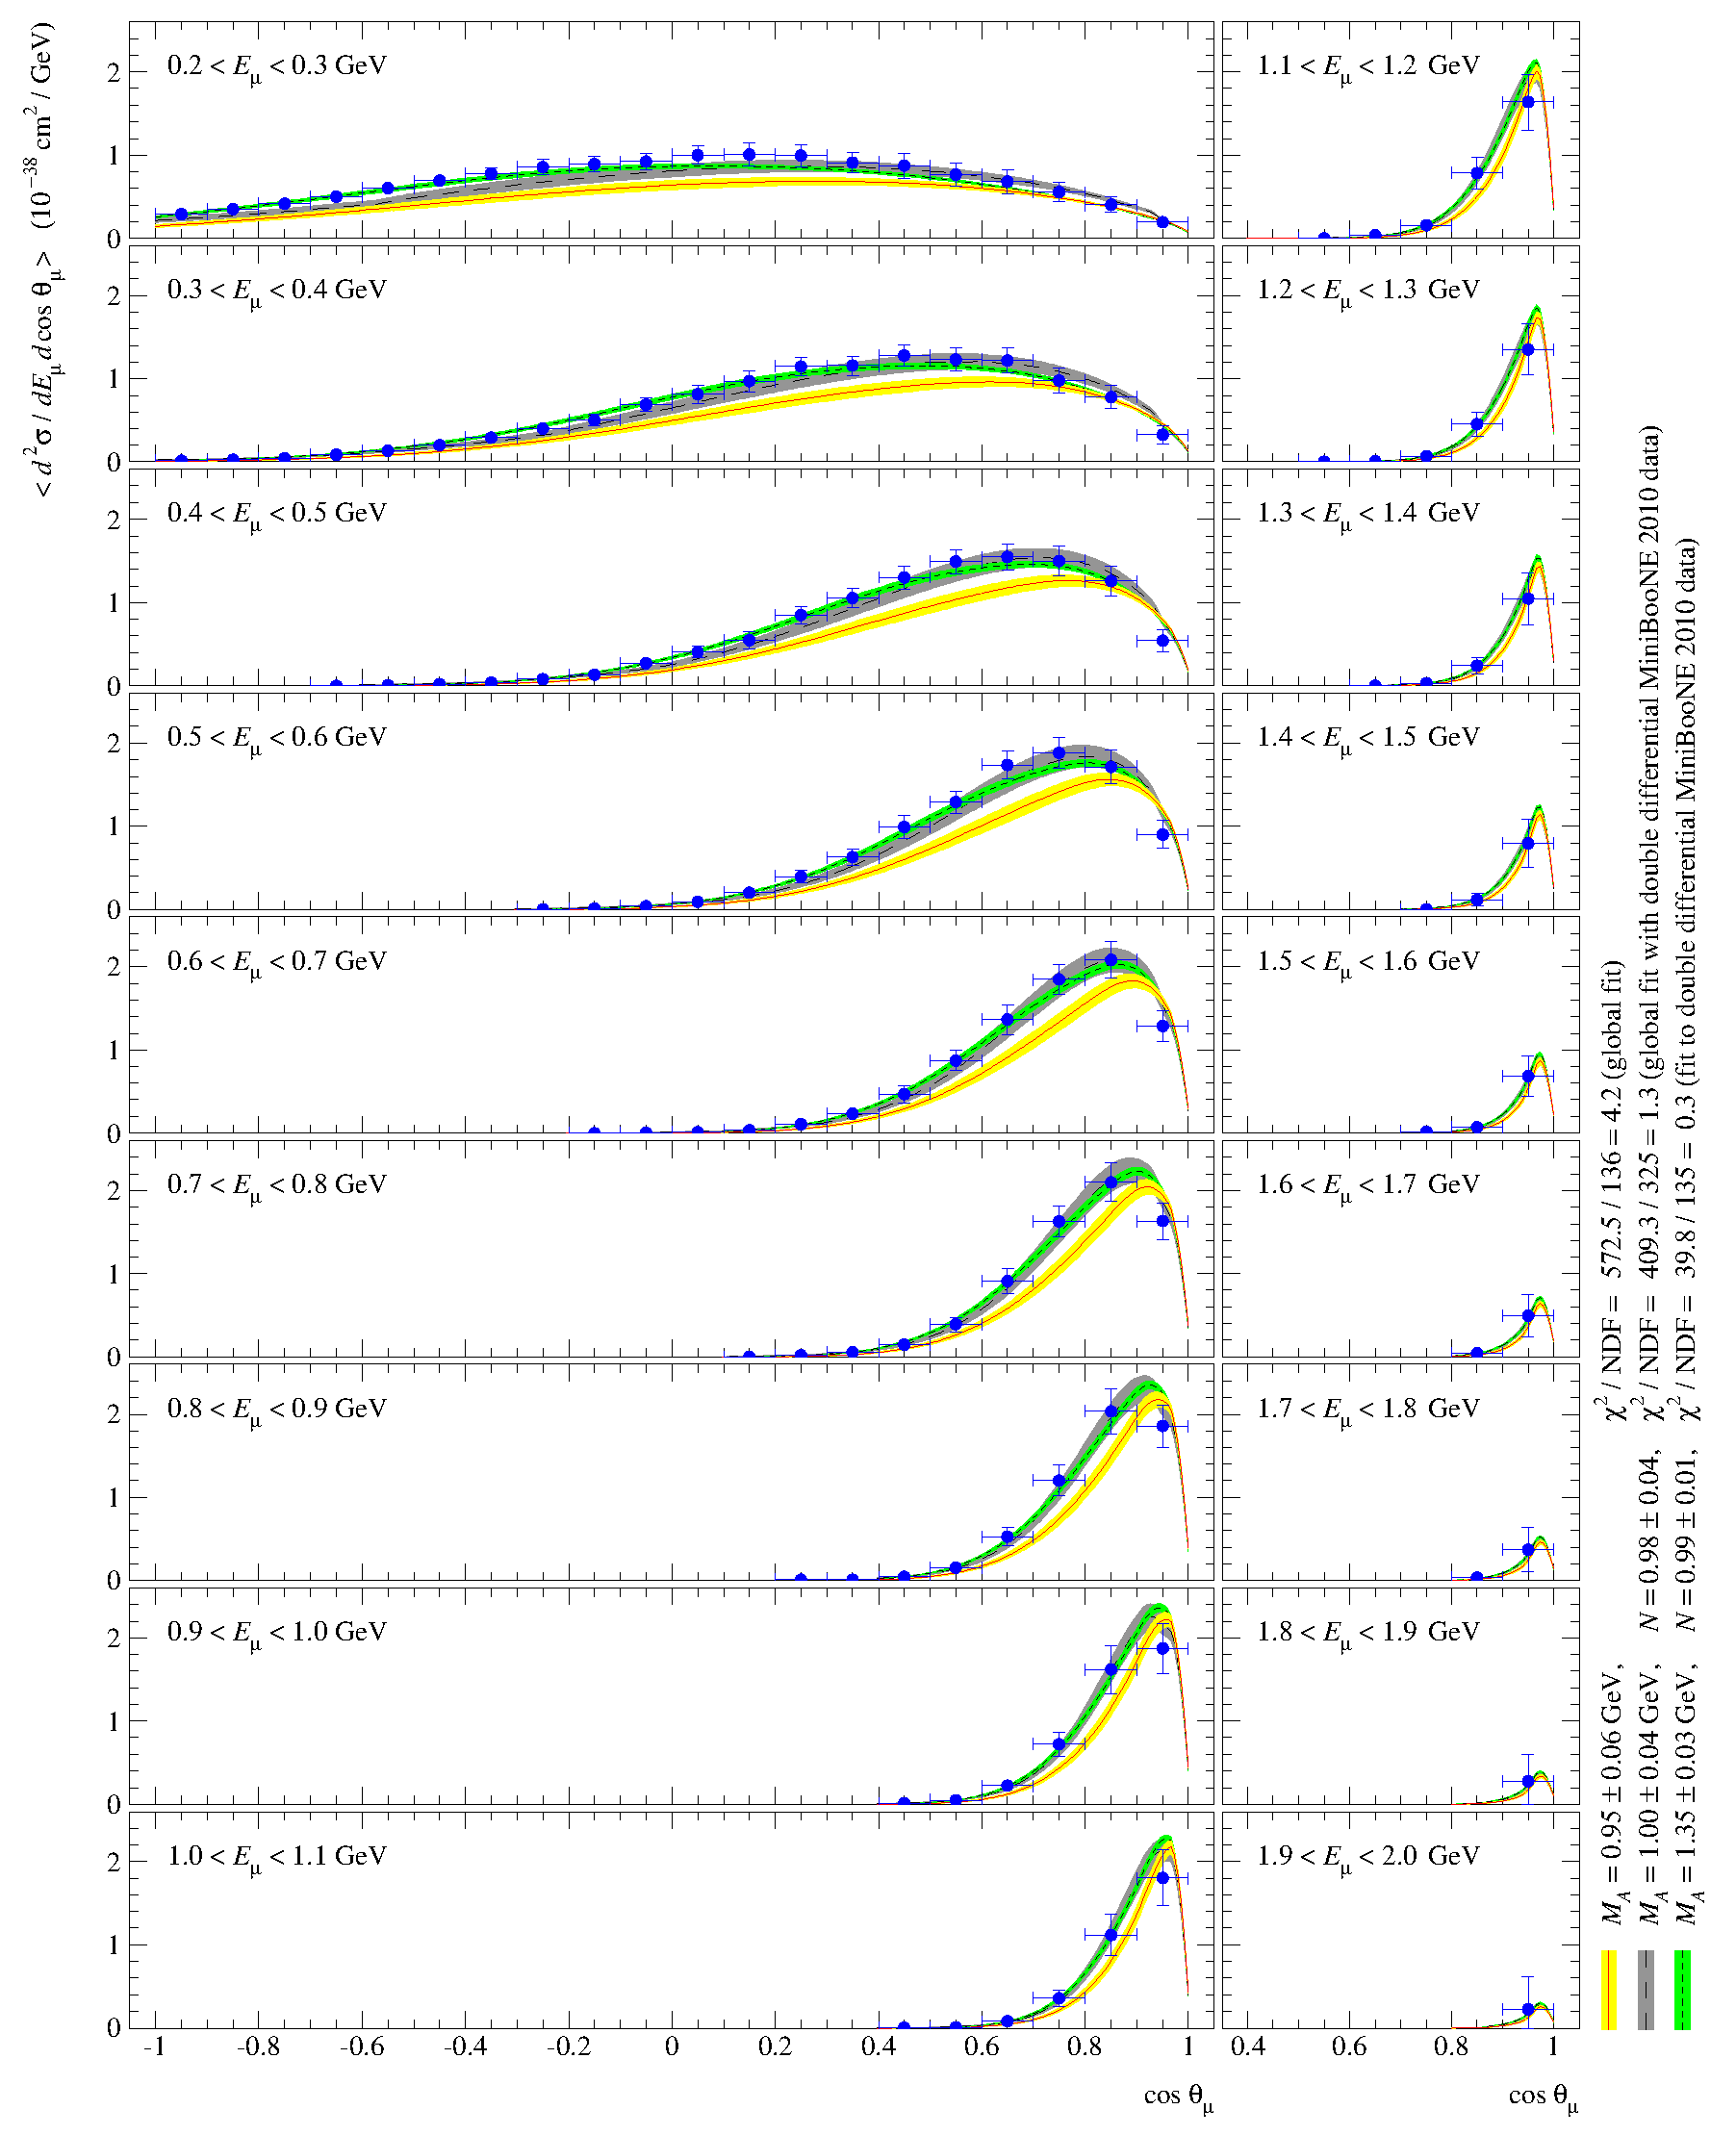
\includegraphics[width=0.5\textwidth]{./QES/d2sQESCC_dEkdcosT_Arevalo_MiniBooNE10_Ek_2_BBBA25.eps}
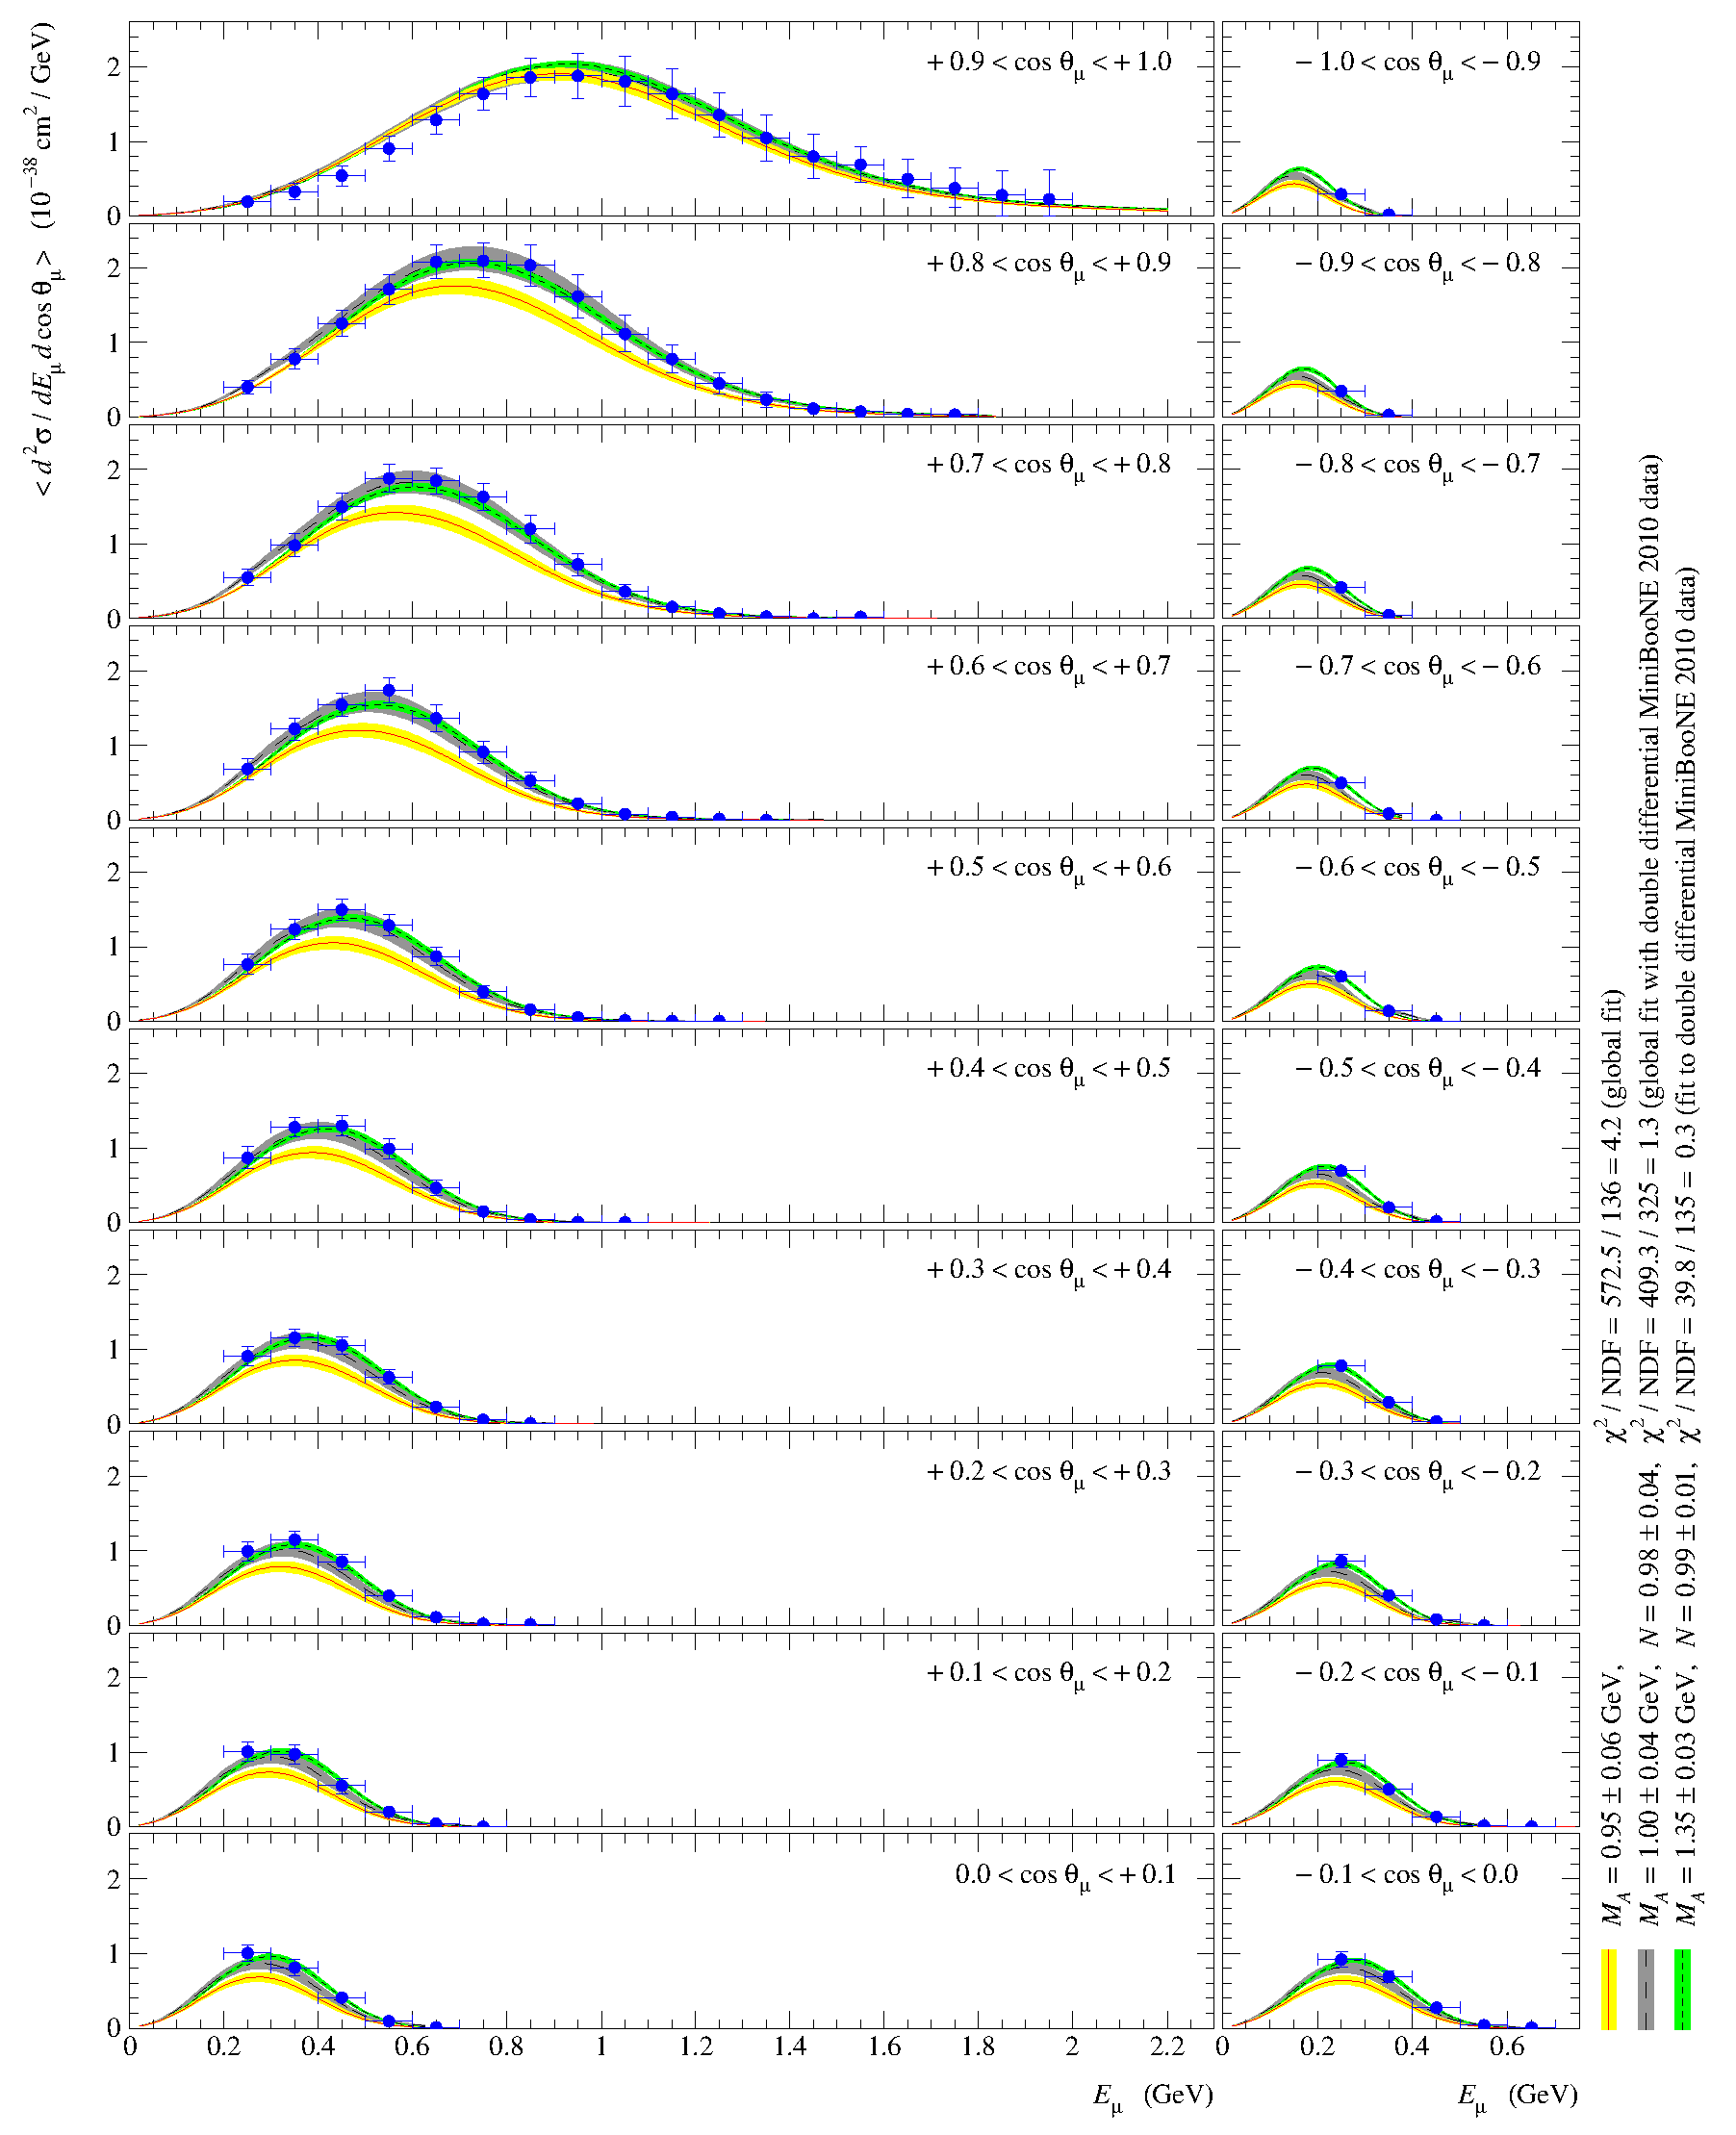
\includegraphics[width=0.5\textwidth]{./QES/d2sQESCC_dEkdcosT_Arevalo_MiniBooNE10_cosT_2_BBBA25.eps}
\caption{\label{MiniBooNE}\textbf{The flux-weighted double differential cross sections} for the $\nu_{\mu}n\to\mu^-p$ reaction measured in the high-statistics experiment MiniBooNE~\cite{AguilarArevalo:2010zc}. The MiniBooNE result: $M_{A}=1.35\pm0.17$\,GeV~\cite{AguilarArevalo:2010zc} is shown by dashed curves corresponding bands. The dark bands are calculated by using the nuclear model of Martini \textit{et al.}~\cite{Martini:2011wp}, \textbf{which yields $M_{A}=1.03$\,GeV} compatible with our best-fit value obtained from high-energy and free-nucleon data}
\end{figure}

Let us stress that the exact knowledge of axial mass is needed for many applications in neutrino physics and astrophysics. In particular, it is important for the data processing of the neutrino oscillation experiments with (anti)neutrinos from accelerators and cosmic rays. The aim of this paper is to investigate the impact of the uncertainty in $M_A$ on the predicted event rates in the underground neutrino detectors. As a major example we consider the World's largest detector Super-Kamiokande.

\section{Methodology: Neutrino fluxes}
\subsection{Atmospheric neutrinos}
Atmospheric neutrinos are produced by the interaction of cosmic rays with the upper atmosphere. In the subsequent calculations we used the 3D Monte Carlo calculations by Honda \textit{et al.}~\cite{Honda:2011nf}. This model is based on the nuclear interaction model JAM used in Particle and Heavy-Ion Transport code System and modified DPMJET-III package. For neutrino fluxes with energy above 10\,GeV we use spectra by Sinegovskaya \textit{et al.}~\cite{Sinegovskaya:2014pia} which is computed by using Hillas-Gaisser cosmic ray spectra~\cite{Gaisser:2013ira} and Kimel-Mokhov hadronic model~\cite{Kalinovsky:1989kk} in semianalytical approach. Figures~\ref{ANspectra} and \ref{ANZAD} represent energy and zenith-angle distributions of atmospheric neutrino fluxes used in this paper.

\begin{figure}[htb!]
\begin{center}
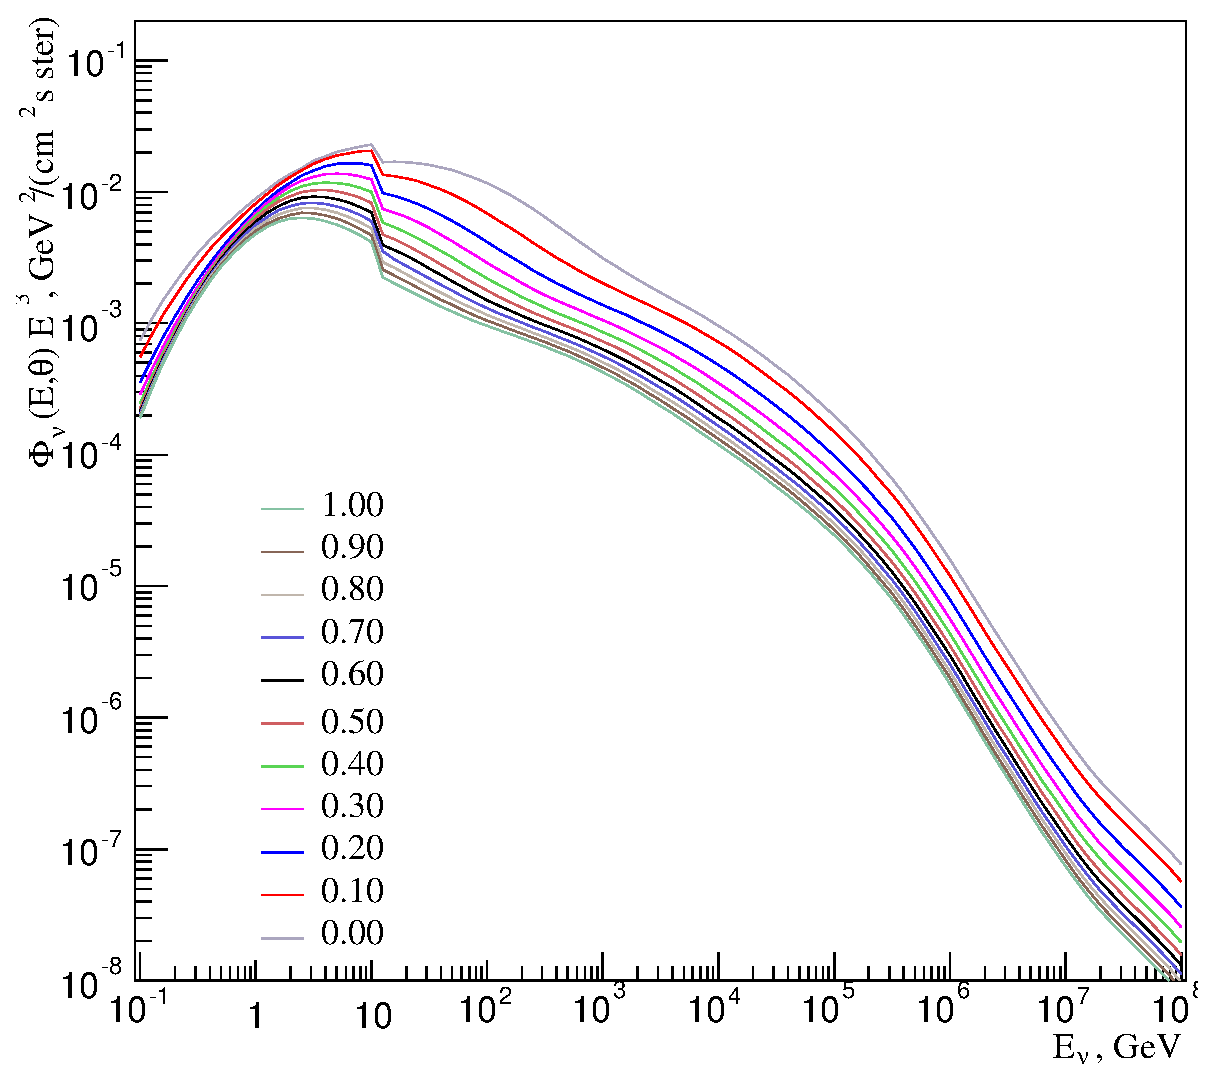
\includegraphics[width=0.45\textwidth]{./AN/HGm_KM_ne_spectra.eps}
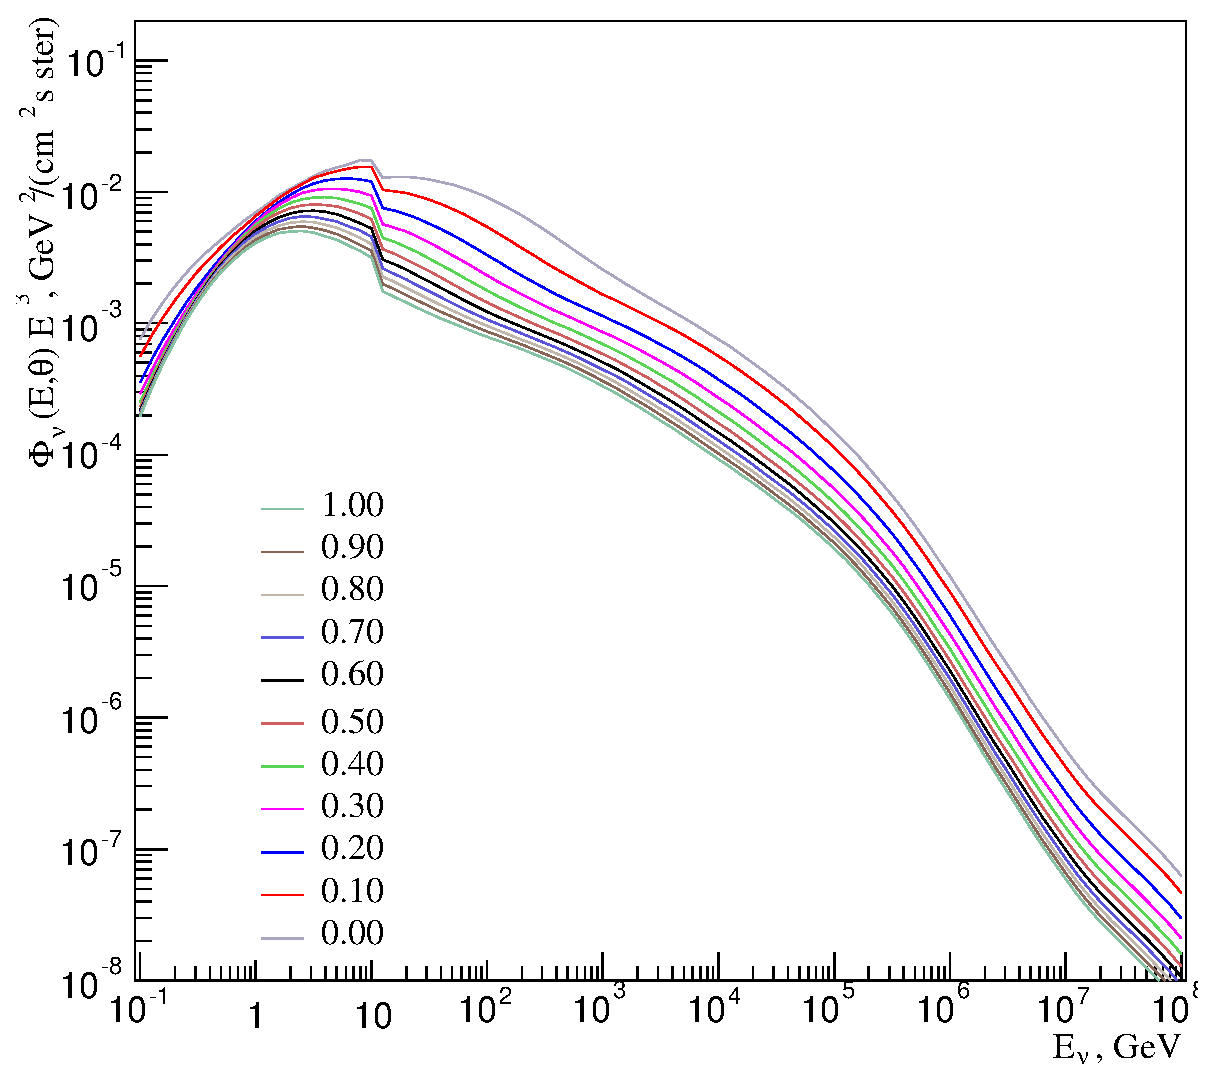
\includegraphics[width=0.45\textwidth]{./AN/HGm_KM_ae_spectra.eps}
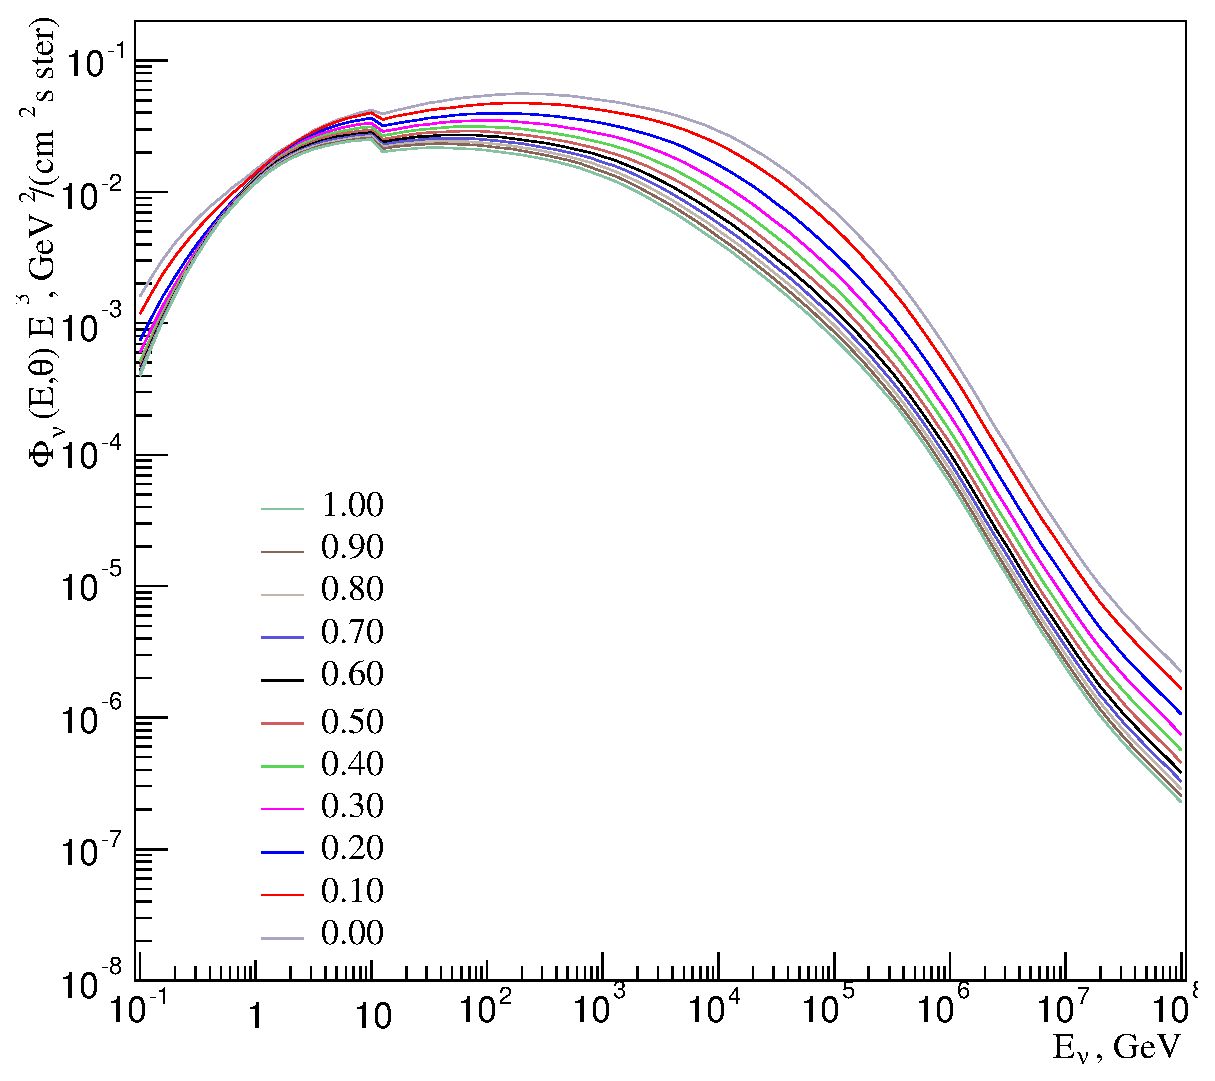
\includegraphics[width=0.45\textwidth]{./AN/HGm_KM_nm_spectra.eps}
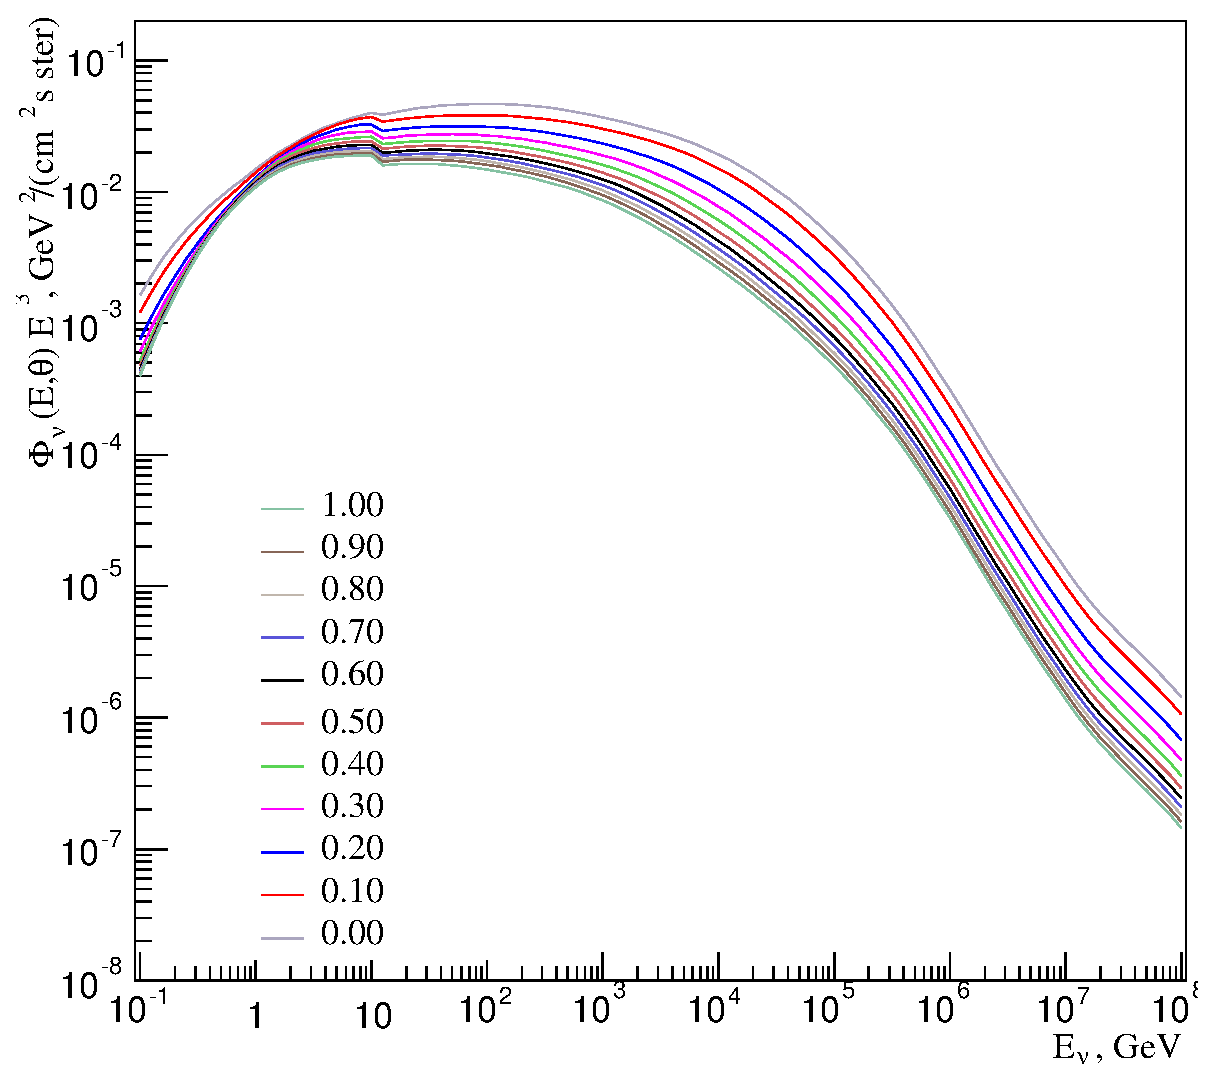
\includegraphics[width=0.45\textwidth]{./AN/HGm_KM_am_spectra.eps}
\caption{\label{ANspectra}Atmospheric neutrino energy spectra by Honda \textit{et al.}~\cite{Honda:2011nf} for $E_{\nu}$ from 100 MeV to 10 GeV and Sinegovskaya \textit{et al.}~\cite{Sinegovskaya:2014pia} for $E_{\nu}$ from 10 GeV to 100 PeV, used in this work}
\end{center}
\end{figure}

\begin{figure}[htb!]
\begin{center}
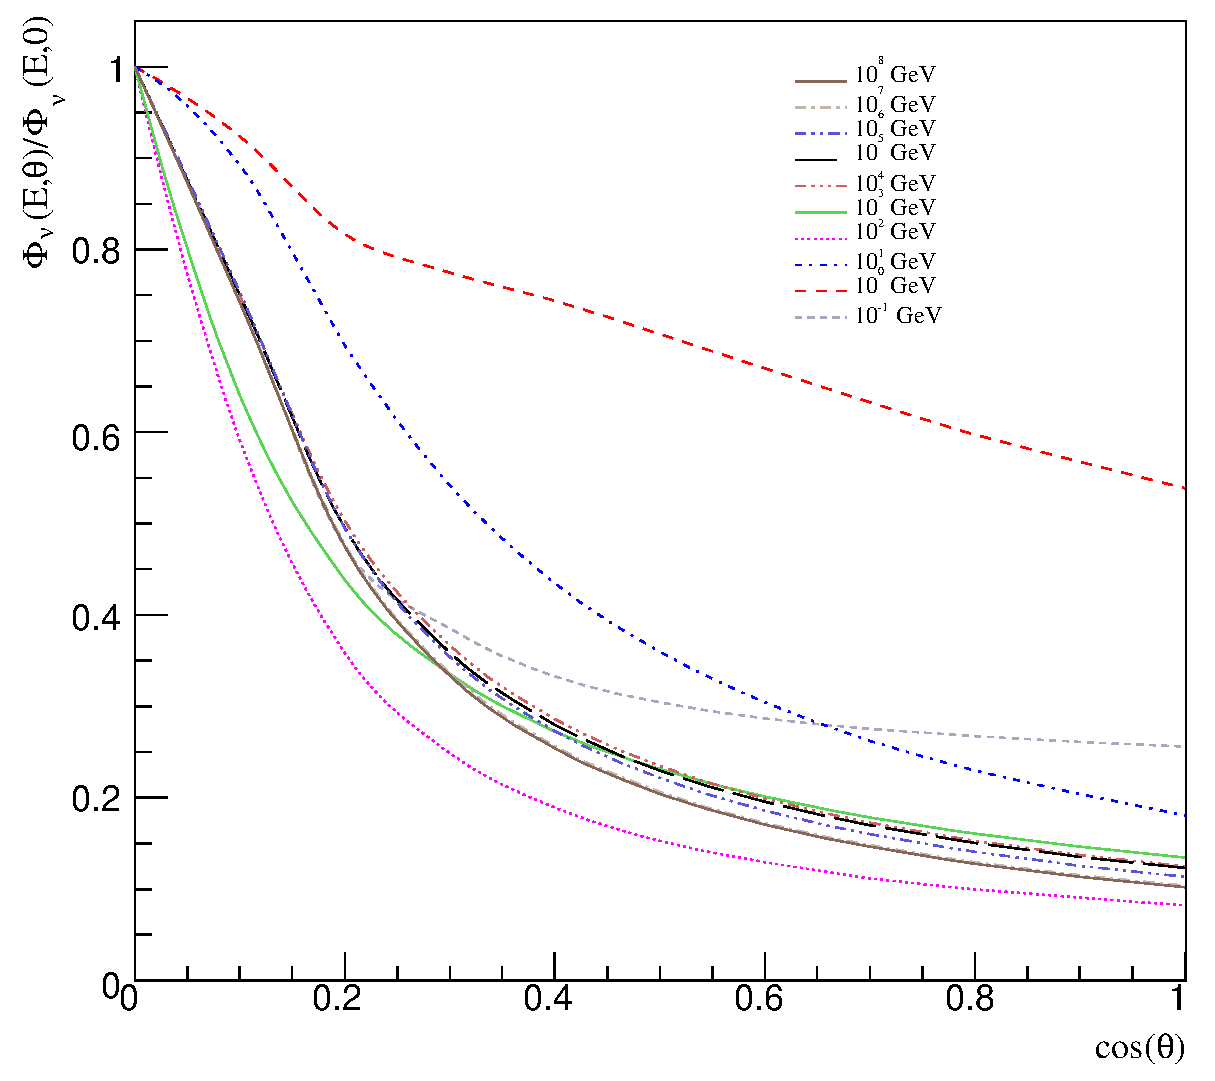
\includegraphics[width=0.45\textwidth]{./AN/HGm_KM_ne_ZAD.eps}
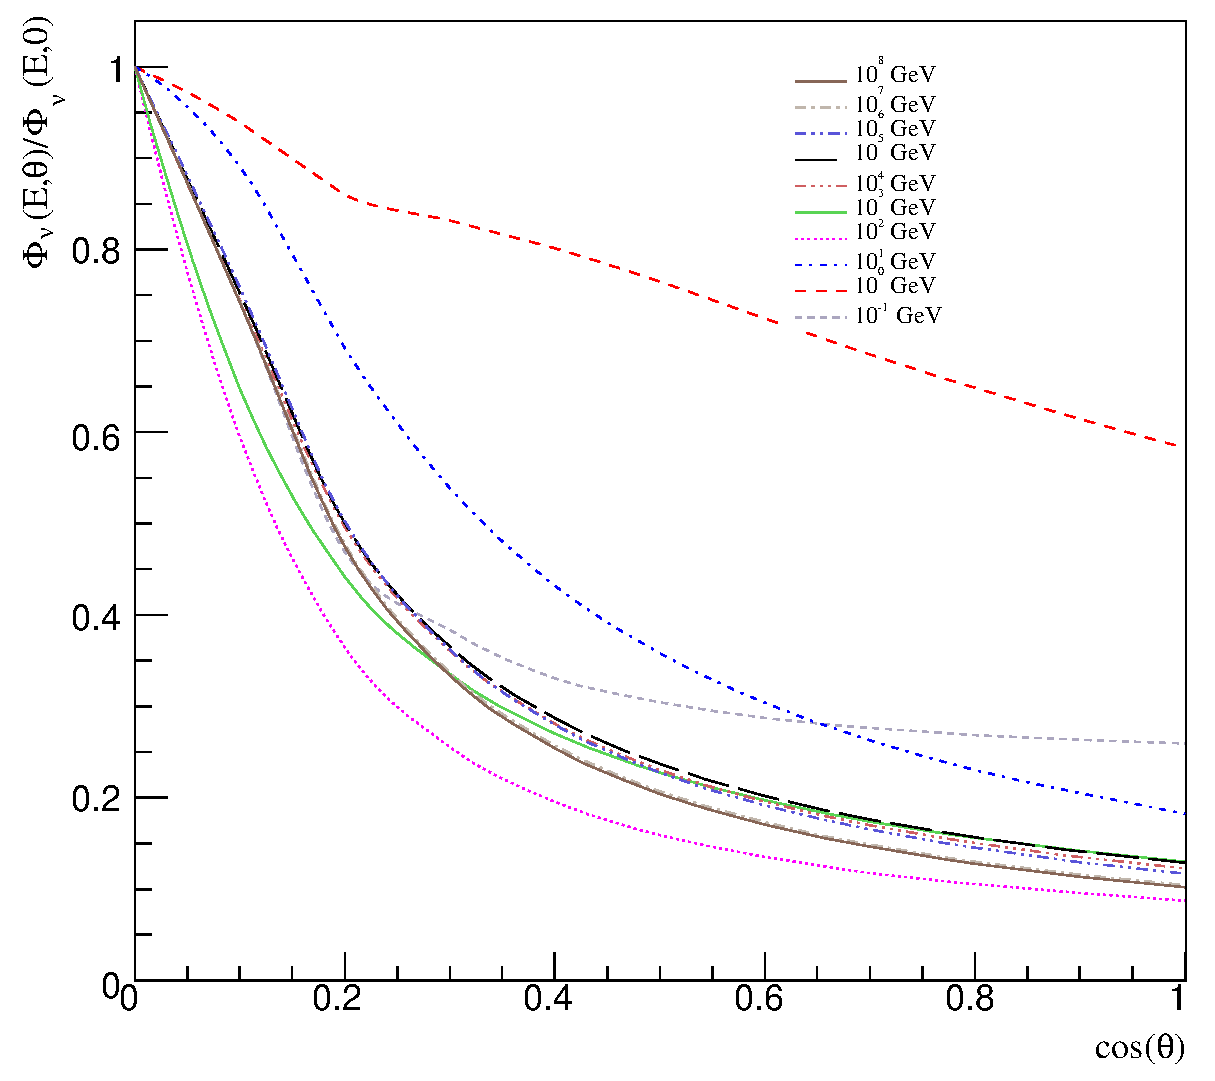
\includegraphics[width=0.45\textwidth]{./AN/HGm_KM_ae_ZAD.eps}
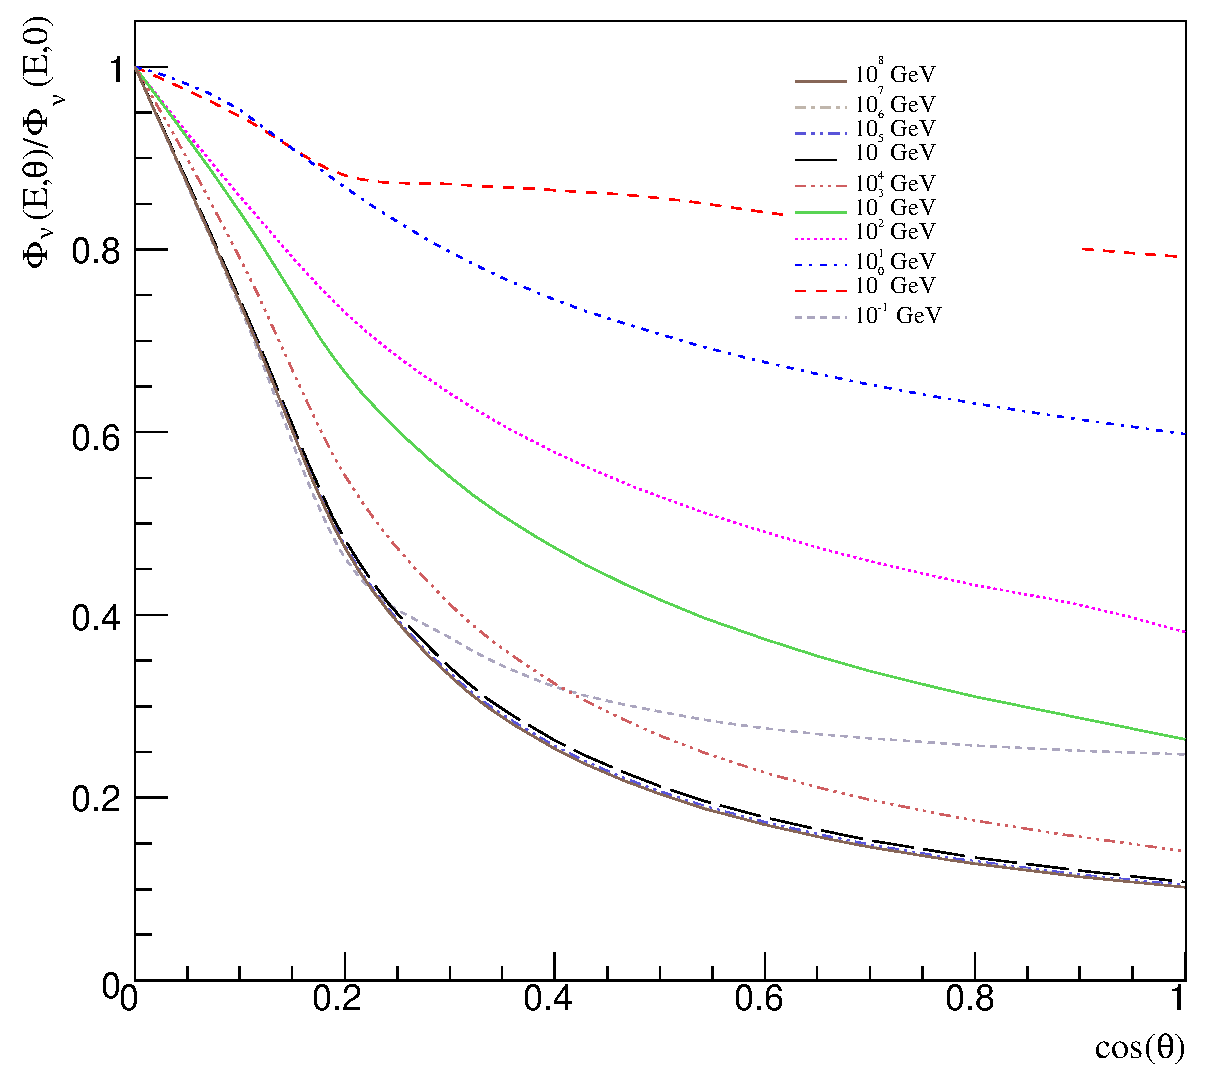
\includegraphics[width=0.45\textwidth]{./AN/HGm_KM_nm_ZAD.eps}
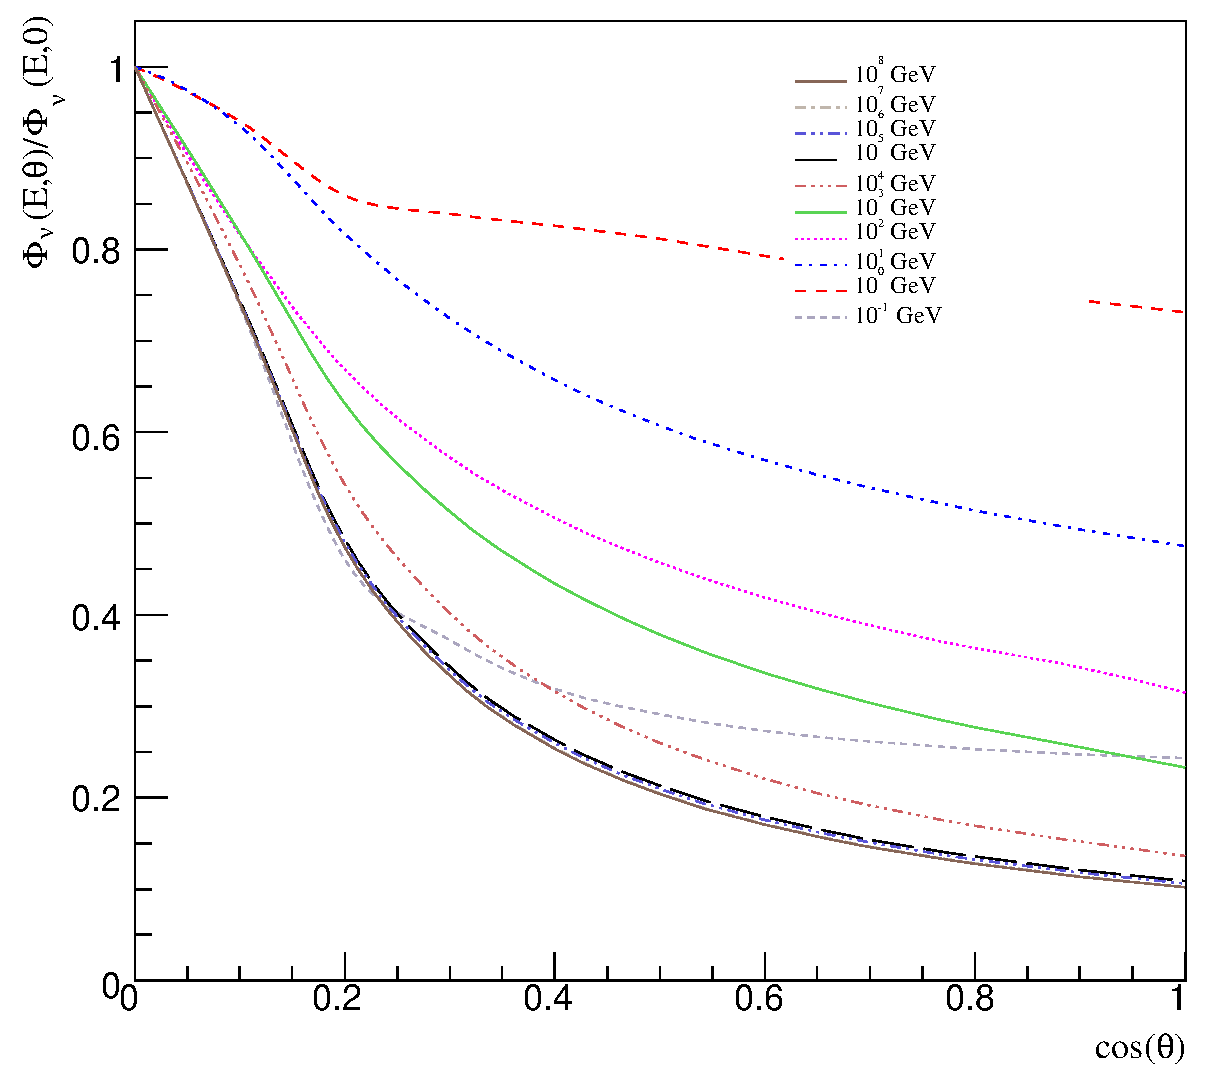
\includegraphics[width=0.45\textwidth]{./AN/HGm_KM_am_ZAD.eps}
\caption{\label{ANZAD}Zenith-angle distributions of atmospheric neutrino fluxes by Honda \textit{et al.}~\cite{Honda:2011nf} for $E_{\nu}$ from 100 MeV to 10 GeV and Sinegovskaya \textit{et al.}~\cite{Sinegovskaya:2014pia} for $E_{\nu}$ from 10 GeV to 100 PeV, used in this work}
\end{center}
\end{figure}

\subsection{Neutrino oscillations in medium}
Atmospheric neutrino fluxes are modified by neutrino oscillation phenomenon. For computing the flavor transition and survival probabilities we applied the result of the global neutrino oscillation data analysis (values of the neutrino mixing angles, CP violating phase and squared mass splittings) by Tortola \textit{et al.}~\cite{Tortola:2012te}.

Before getting the detector, atmospheric neutrinos pass through the body of the Earth. Therefore, we had to take into account the neutrino-matter coherent scattering (MSW effect). To solve the Wolfenstein equations describing the evolution of the neutrino system in a medium we decided to adopt the method from work~\cite{Naumov:2001ci}.

The density profile in the Earth in the presented calculations is described according to the Preliminary Reference Earth Model (PREM)~\cite{Dziewonski:1981xy} which contains 10 layers of density with various behaviour~\ref{PREM}. According to the method, each layer with varying density must be split into a number of sublayers of conditionally constant density. Hereby the process of neutrino propagating, from the moment of its birth in the sourse to the moment of entering the detector, may be considered as a process of consecutive propagations through a number of segments of relatively invariable density. Thus if ${S_{i}}$ is the evolution operator and the solution of Wolfenstein equation for the system of three mixed Dirac neutrinos passing through the $i$-th segment with constant density then $S=\prod{S_{i}}$ is the solution for the whole path from the source to the detector.

\begin{figure}[htb!]
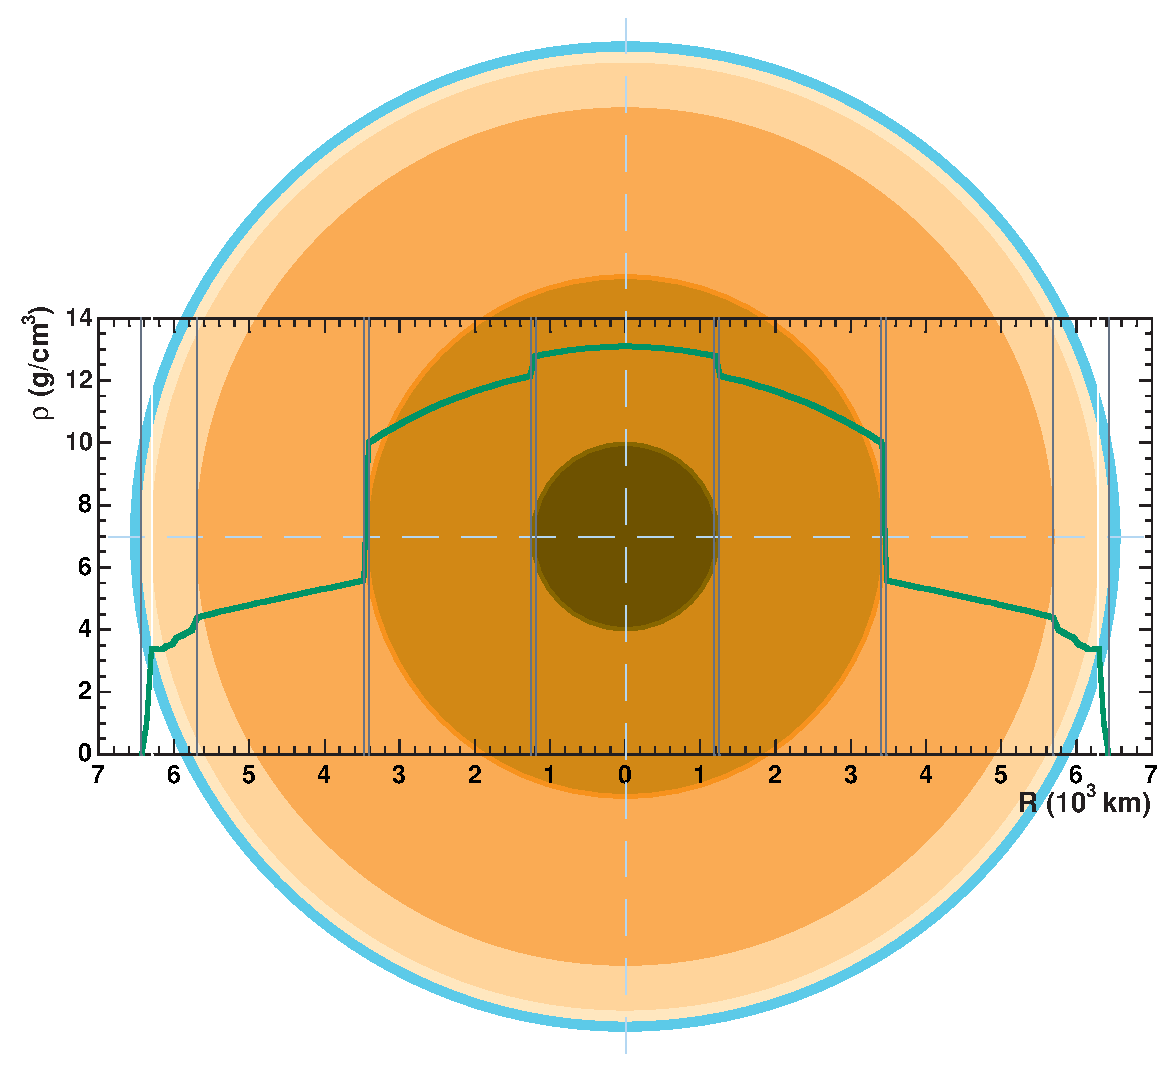
\includegraphics[width=0.5\textwidth]{./MSW/Earth_PREM.eps}
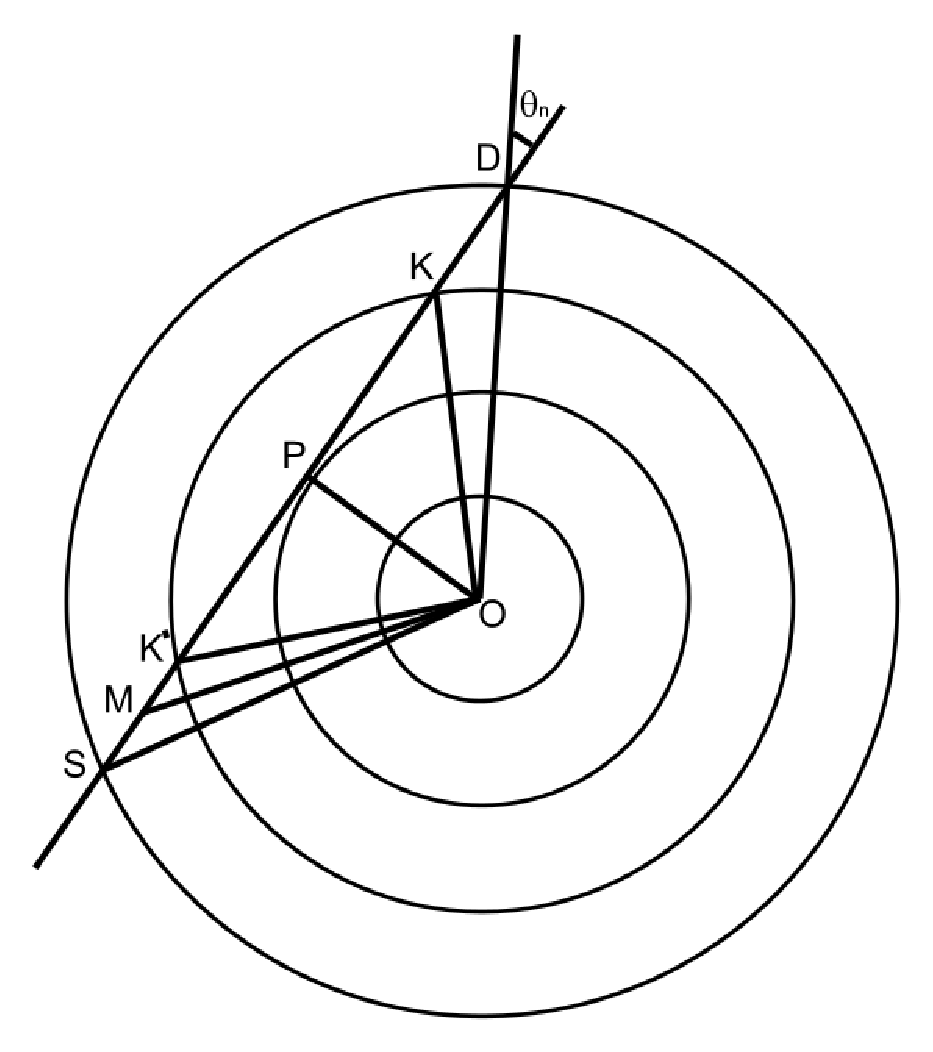
\includegraphics[width=0.5\textwidth]{./MSW/Earth_Layers.eps}
\caption{\label{PREM}Preliminary Reference Earth Model (PREM)~\cite{Dziewonski:1981xy} and the method of sublayers}
\end{figure}

The convenience of such method follows from the fact that independently of density distribution in a medium we have to find an exact solution of the equation for constant density only. Such solution has been obtained in work~\cite{Naumov:1991ju,Naumov:1991rh}. It is also worth noticing here that the number of sublayers in each layer is, by virtue of different thickness of such layers, individual and regulated by a convergence criterion for the method used. The criterion itself states that there're numbers ${N_{i}}$ of segments that each $i$-th layer is split into such that further increasing of these numbers doesn't change the values of probabilities within the desired accuracy. In our case these numbers can be established numerically only.

Examples of the neutrino oscillogramms in the Earth you can see in Fig.~\ref{ogramms}. Figure~\ref{modspectra} shows atmospheric neutrino spectra modulated neutrino oscillations in the Earth matter.

\begin{figure}[htb!]
\begin{center}
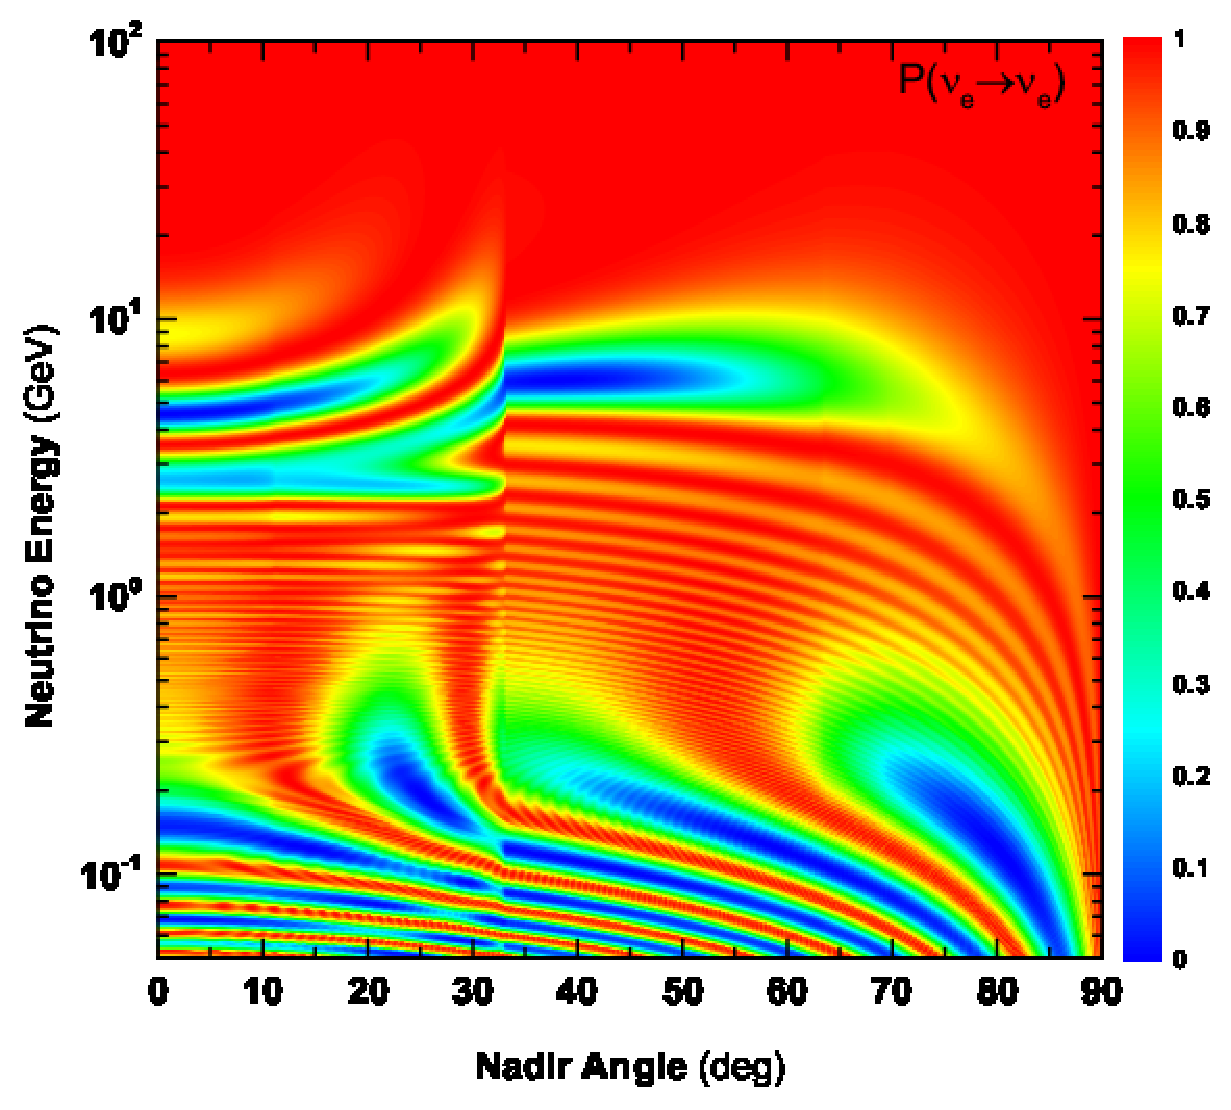
\includegraphics[width=0.3\textwidth]{./MSW/Pee-NH2.eps}
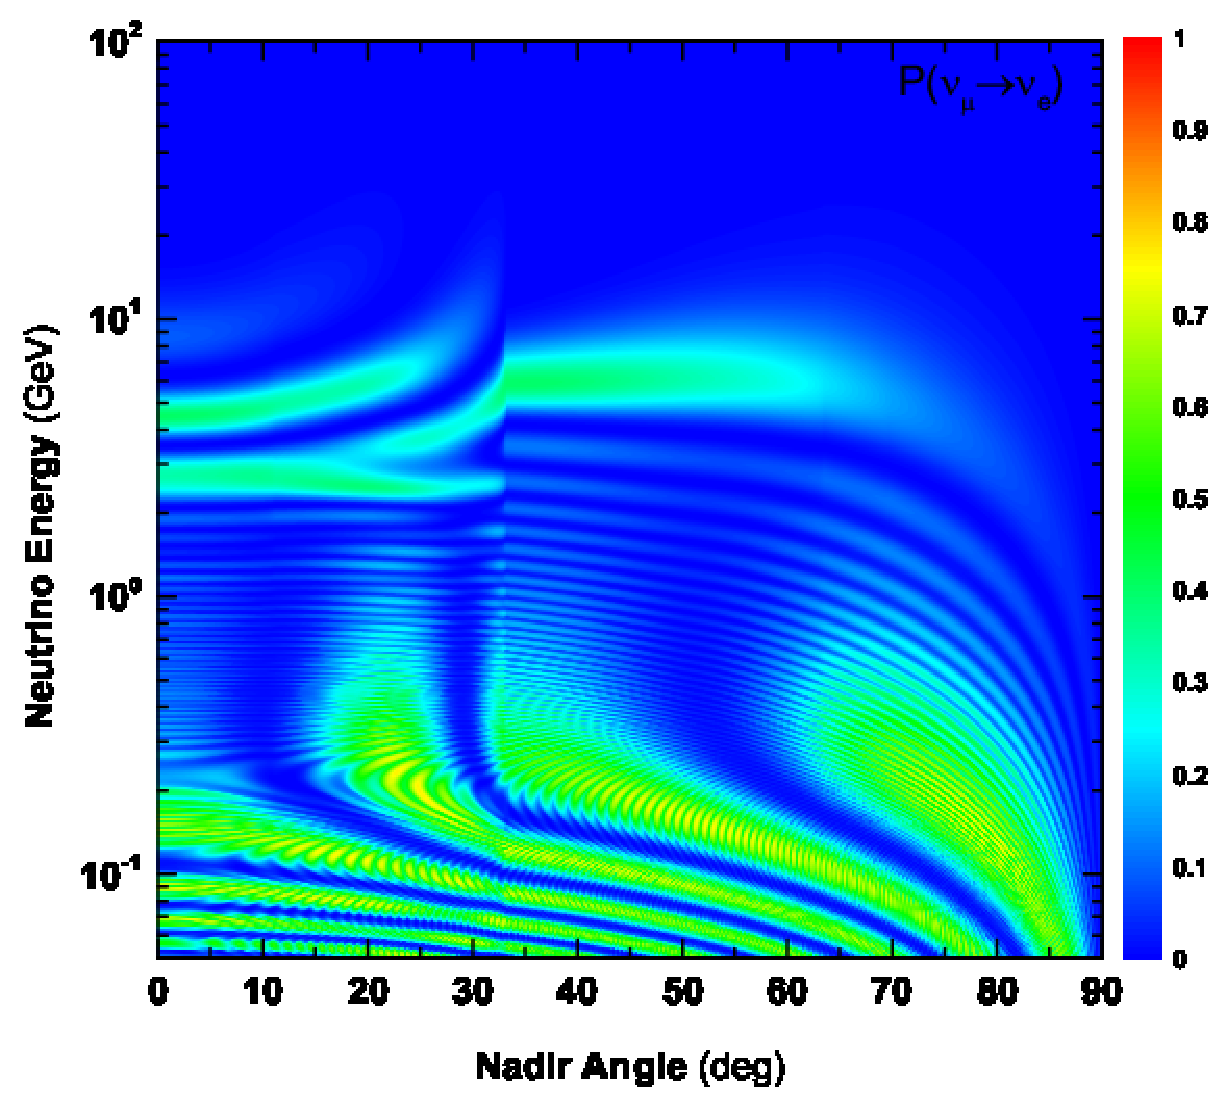
\includegraphics[width=0.3\textwidth]{./MSW/Pme-NH2.eps}
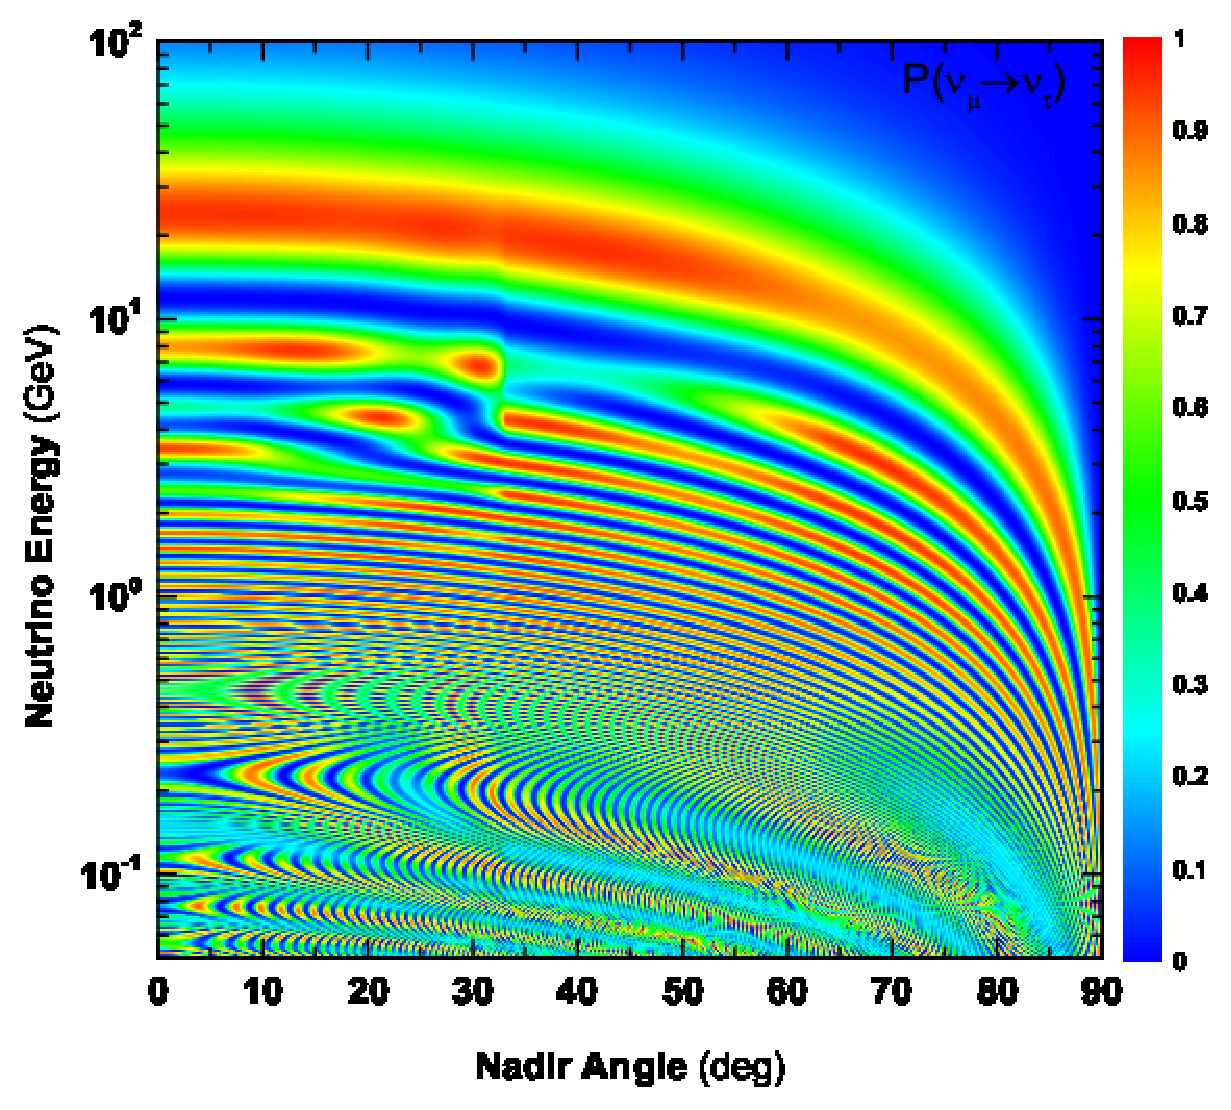
\includegraphics[width=0.3\textwidth]{./MSW/Pmt-NH2.eps}
\caption{\label{ogramms}\textbf{Neutrino oscillogramms} in the Earth for the case of normal neutrino mass, left to right: $\nu_{e}$ survival probability plot, $P_{\nu_{\mu}}\to{}P_{\nu_{e}}$, $P_{\nu_{\mu}}\to{}P_{\nu_{\tau}}$}
\end{center}
\end{figure}

\begin{figure}[htb!]
\begin{center}
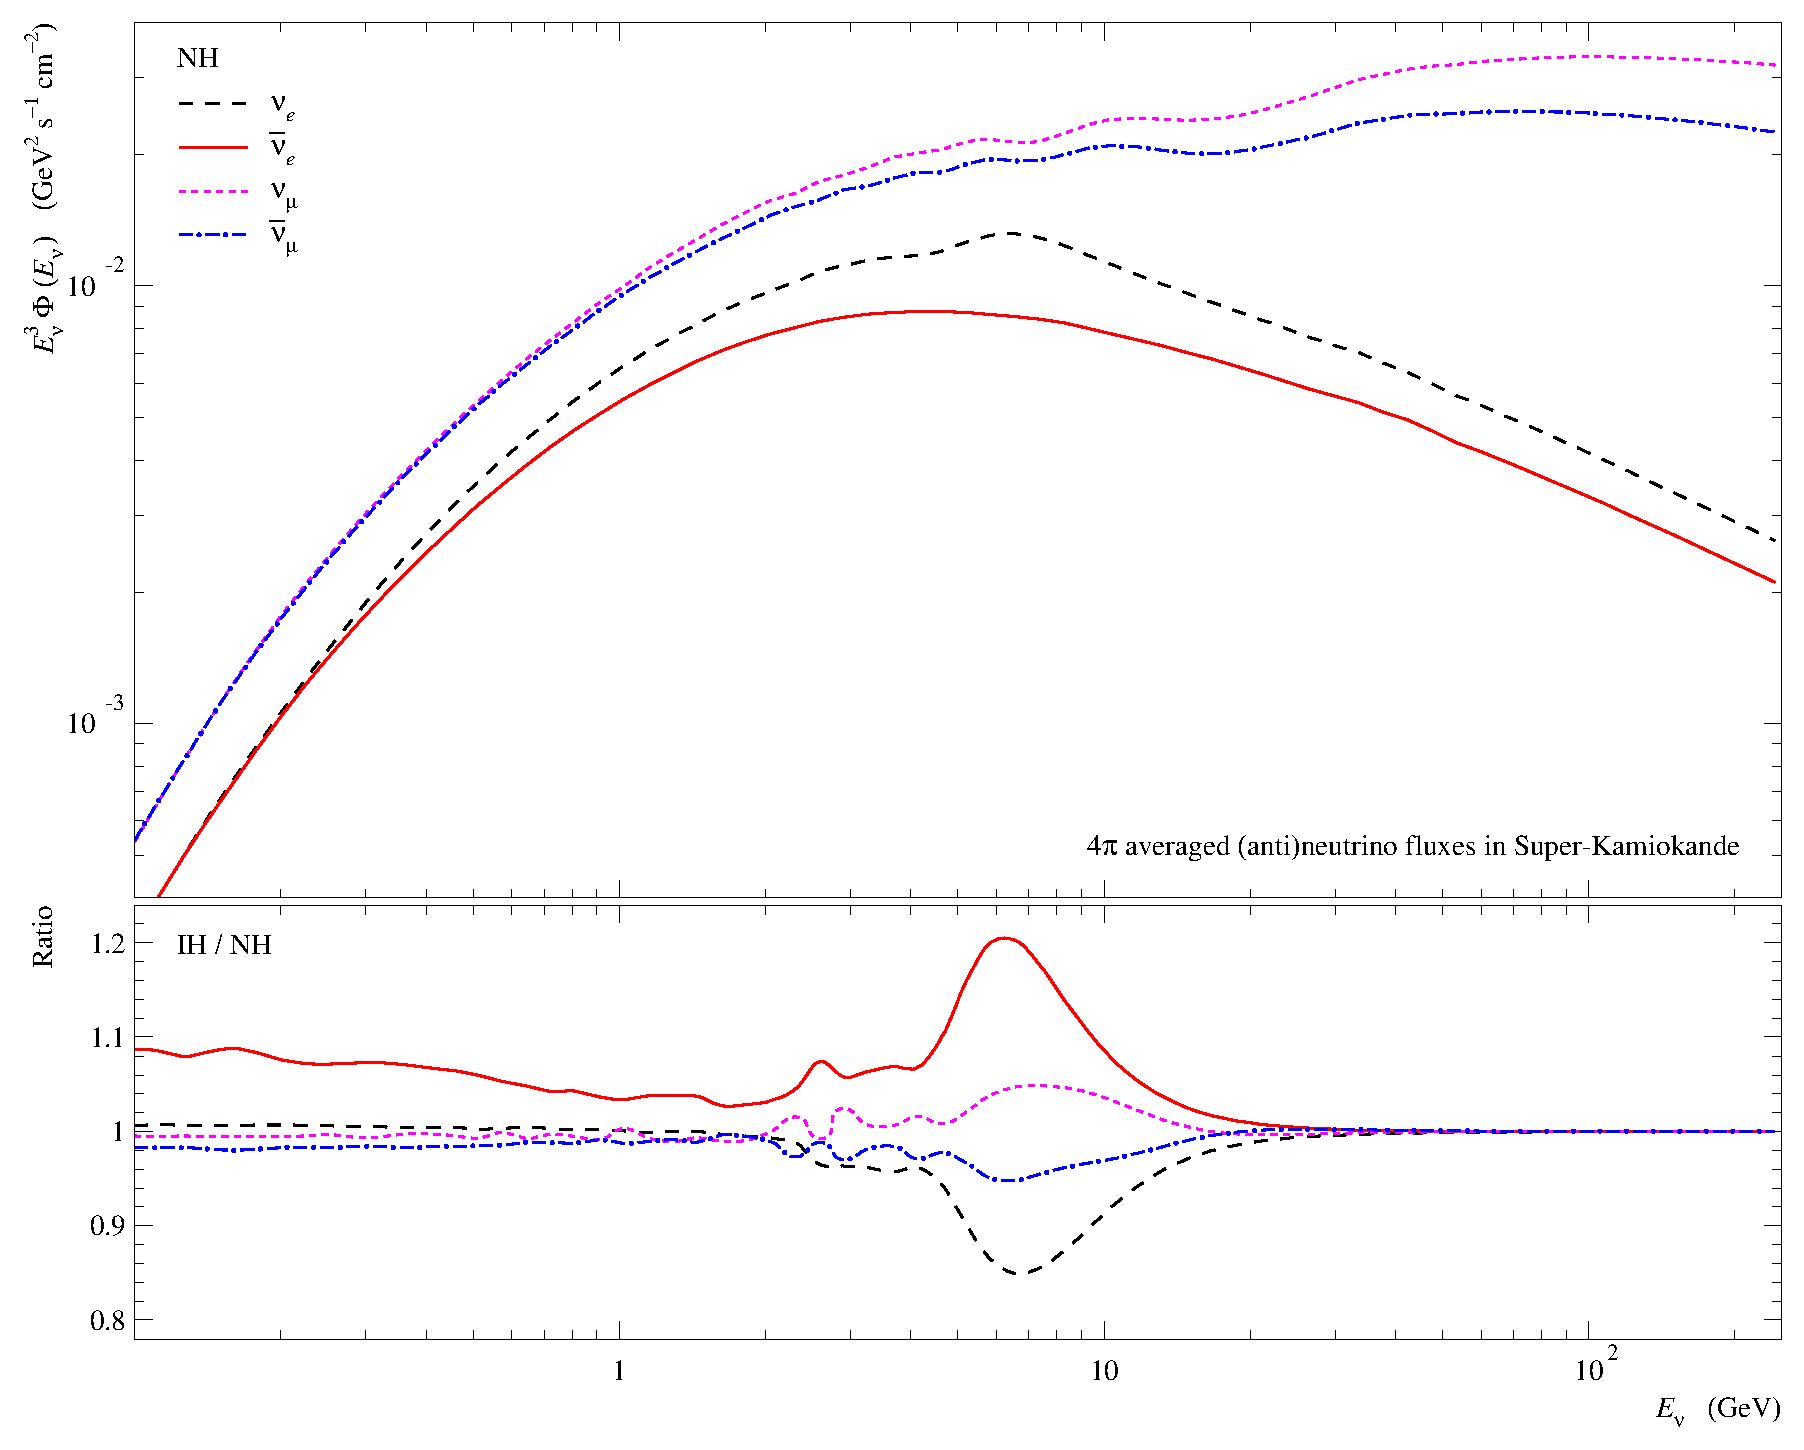
\includegraphics[width=0.6\textwidth]{./MSW/dF_dE_Honda11.eps}
\caption{\label{modspectra}\textbf{Flavor transition modulated} $4\pi$-averaged energy spectra of atmospheric neutrinos in Super-Kamiokande for the normal neutrino mass hierarchy (top panel) and the ratios of the energy spectra for the inverse mass hierarchy to these for the normal mass hierarchy (bottom panel)}
\end{center}
\end{figure}

Neutrino oscillations in NO$\nu$A are mostly caused by MSW effect. The maximal depth of neutrino beam is about 10\,km. So, for calculations the equation for constant density medium is sufficiently. MC for neutrino fluxes in the NOvA experiment is shown in Fig.~\ref{NOvAspectra}.

\begin{figure}[htb!]
\begin{center}
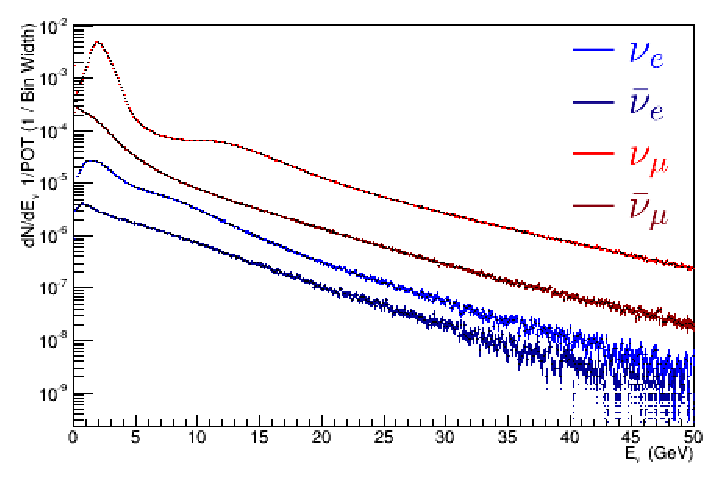
\includegraphics[width=0.45\textwidth]{./NOvA/ND_n.eps}
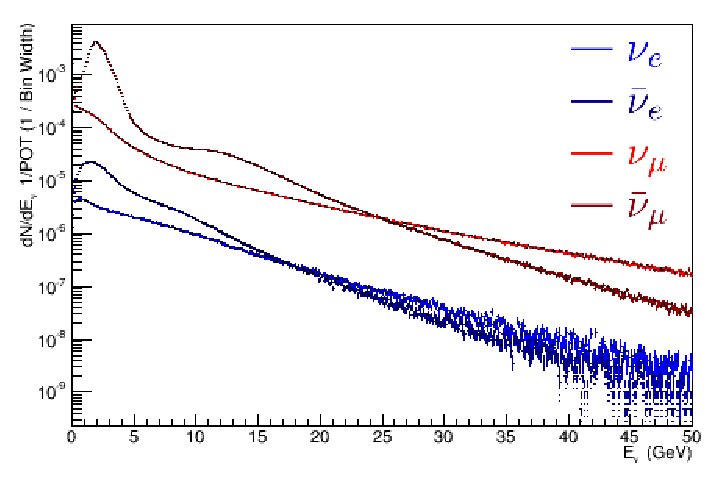
\includegraphics[width=0.45\textwidth]{./NOvA/ND_a.eps}
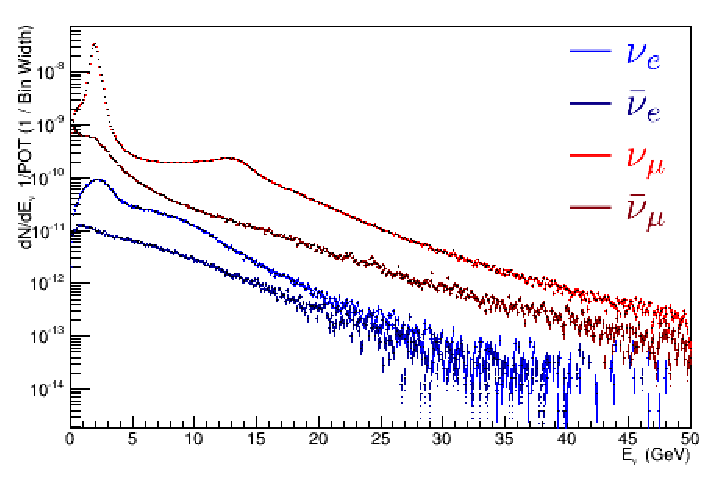
\includegraphics[width=0.45\textwidth]{./NOvA/FD_n.eps}
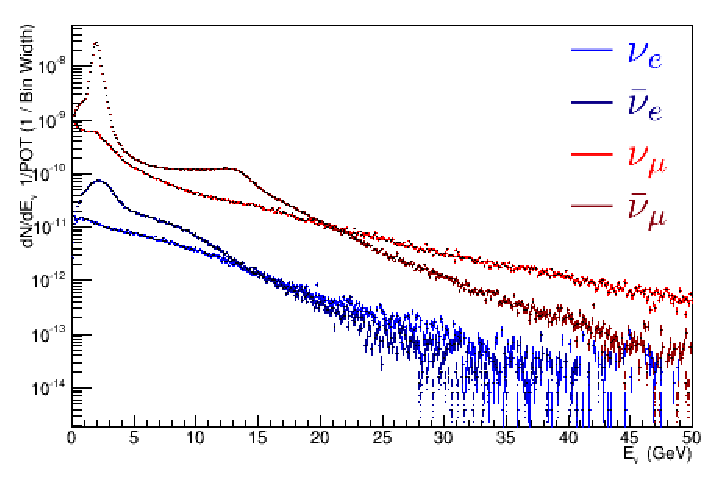
\includegraphics[width=0.45\textwidth]{./NOvA/FD_a.eps}
\caption{\label{NOvAspectra}Neutrino fluxes in the NOvA experiment, left-to-right: $\nu$ and $\bar\nu$-beam in Near (Far) Detector (top (bottom) panel)}
\end{center}
\end{figure}

\section{Methodology: Quasielastic neutrino-nucleus cross sections}
\subsection{The nuclear model problem}
Currently there is no generally accepted model for calculating neutrino-nucleus interaction cross sections, applicable in a wide energy range from threshold to ultrahigh values. The importance of the choice of nuclear physics model for neutrino oscillations is considered in the work by Meloni and Martini~\cite{Meloni:2012fq}, where the results of the experiment T2K~\cite{Abe:2011sj,Abe:2012gx} retrieves the value of the neutrino mixing parameters with using conventional Relativistic Fermi gas model (RFG), as well as MECM model~\cite{Martini:2009uj}. The most striking difference is observed for the angle $\theta_{13}$: $\sin^{2}2\theta_{13}^{\textrm{RFG}}=0.138^{+0.031}_{-0.041}$ is approximately $1.5$ times bigger than $\sin^{2}2\theta_{13}^{\textrm{MECM}}=0.092^{+0.030}_{-0.052}$.

All of experimantal data mentioned in Introduction have been obtained by using RFG model. Applying another model could essentially modify extracted values including nucleon axial mass. Figure~\ref{MiniBooNE} demonstrates that nuclear model of Martini~\textit{et al.} can describe MiniBooNE data~\cite{AguilarArevalo:2010zc} with $M_{A}=1.03$\,GeV~\cite{Martini:2011wp}. At high energies nuclear effects are less important, that explains good agreement between experimental data and RFG model with $M_{A}=1.012\pm{0.031}$\,GeV~\cite{Kuzmin:2014}. Hydrogen and deuterium calculations don't use nuclear model at all and gives us $M_{A}=1.026\pm{0.031}$\,GeV~\cite{Kuzmin:2014}. $M_{A}$ extracted in both these cases are consistent with each other and with result of Martini~\textit{et al.}. K2K and T2K experiments that are not agree with $M_{A}\sim1$\,GeV, deal with lower neutrino energies too. The natural conclusion is that RFG model used for data processing in experiments does not work at low energies.

The problem is that there is no nuclear model which works properly for all energies. Therefore, even in case the correct value of the axial mass was known, using it with wrong nuclear model could not describe experimental data on quasielastic cross sections and would lead to errors in predictions.

\subsection{The effective axial mass approach}
Phenomenological solution of this problem is as follows. As we know, using RFG model with different values of $M_{A}$ can give a good description of experimental data obtained in different energy ranges. Thus, we propose to continue using this model but modify the axial form factor to compensate nuclear effects in the low-energy region. For this parametrization we need to introduce the variable effective axial mass as a function of neutrino energy and use it instead of conventional constant $M_{A}$. Of course, modified functions $F_{A}^\mathrm{eff}(Q^{2},E_{\nu})$, $F_{P}^\mathrm{eff}(Q^{2},E_{\nu})$, which defined by~(\ref{formfactors}) with $M_{A}$ replaced by $M_{A}^\mathrm{eff}$, are no longer axial-vector and pseudoscalar form-factors.

Figure~\ref{MA_QES_eff} demonstrates how one can fit experimental data to get the $M_{A}^\mathrm{eff}$. We chose for parameterization a simple form:
\begin{equation}
M_{A}^\mathrm{eff}=M_{0}\left(1+\frac{E_{0}}{E_{\nu}}\right).
\end{equation}
Global analysis of the experimental data on total and differential quasielastic neutrino cross-sections gives us the following values of parameters:
\begin{equation}
M_{0}=1.019\pm0.027\pm0.032\,\mathrm{GeV},
\end{equation}
\begin{equation}
E_{0}=0.327\tbinom{+0.060}{-0.056}\tbinom{+0.072}{-0.067}\,\mathrm{GeV},
\end{equation}
where $1\sigma$ and $2\sigma$ errors are shown.

\begin{figure}[htb!]
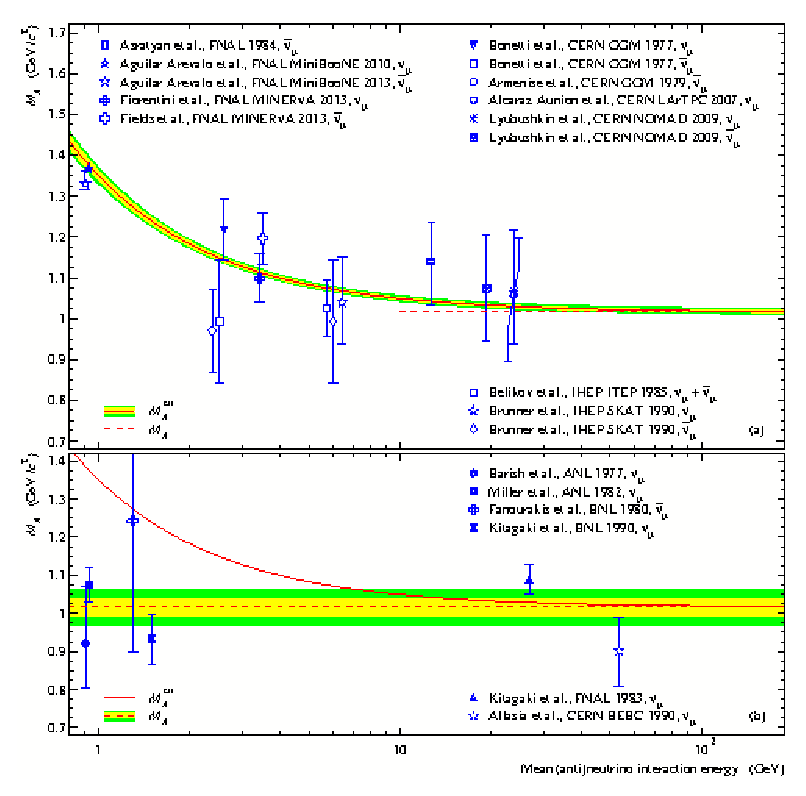
\includegraphics[width=\columnwidth]{./QES/MA_QES_eff.eps}
\caption{\label{MA_QES_eff}Fitting experimental data for $M_{A}^\mathrm{eff}$ parameterization. Only selected data are shown}
\end{figure}

In Fig.~\ref{TotalCS} it is shown, that data obtained in experiments with hydrogen and deuterium do not contradict with the best-fit constant axial mass. But MiniBooNE and, for example, NOMAD datasets are not consistent in any constant $M_{A}$ hypothesis. On the contrary, applying the offered $M_{A}^\mathrm{eff}$ gives a good description of these experiments. Please, pay attention on the fact that the flux energy peak of NO$\nu$A experiment lays between their studied areas as well as energy range of most of the fully-contained events in Super-Kamiokande.

\section{Results and discussion: The axial mass effect}
Figure~\ref{SKrates} displays the result of our calculation: ratios of the neutrino event rates caused by the QES interactions with hydrogen and oxygen nuclei in the Super-Kamiokande detector, evaluated with several values of conventional constant $M_{A}$ to ones computed with preliminary offered $M_{A}^{\mathrm{eff}}$. Figure~\ref{NOvArates} presents results for NO$\nu$A experiment in analogical way.

\begin{figure}[htb!]
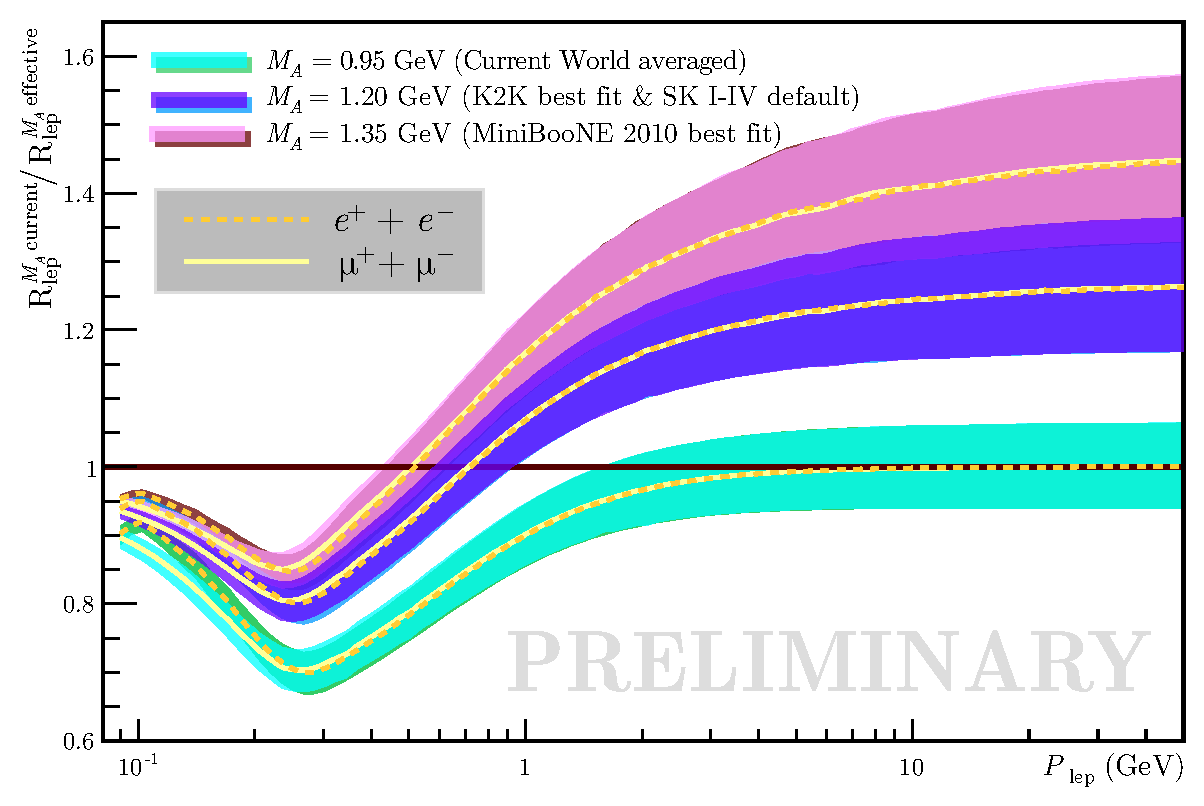
\includegraphics[width=\columnwidth]{./SK/cvsv2lmn_all2.eps}
\caption{\label{SKrates}Electron-like and muon-like event rates caused by the QES interactions in the Super-Kamiokande detector. The rates are evaluated with several constant values of $M_{A}$ and normalized to the rates calculated with $M_{A}^{\mathrm{eff}}$. The calculations are done for the normal neutrino mass hierarchy}
\end{figure}

\begin{figure}[htb!]
\begin{center}
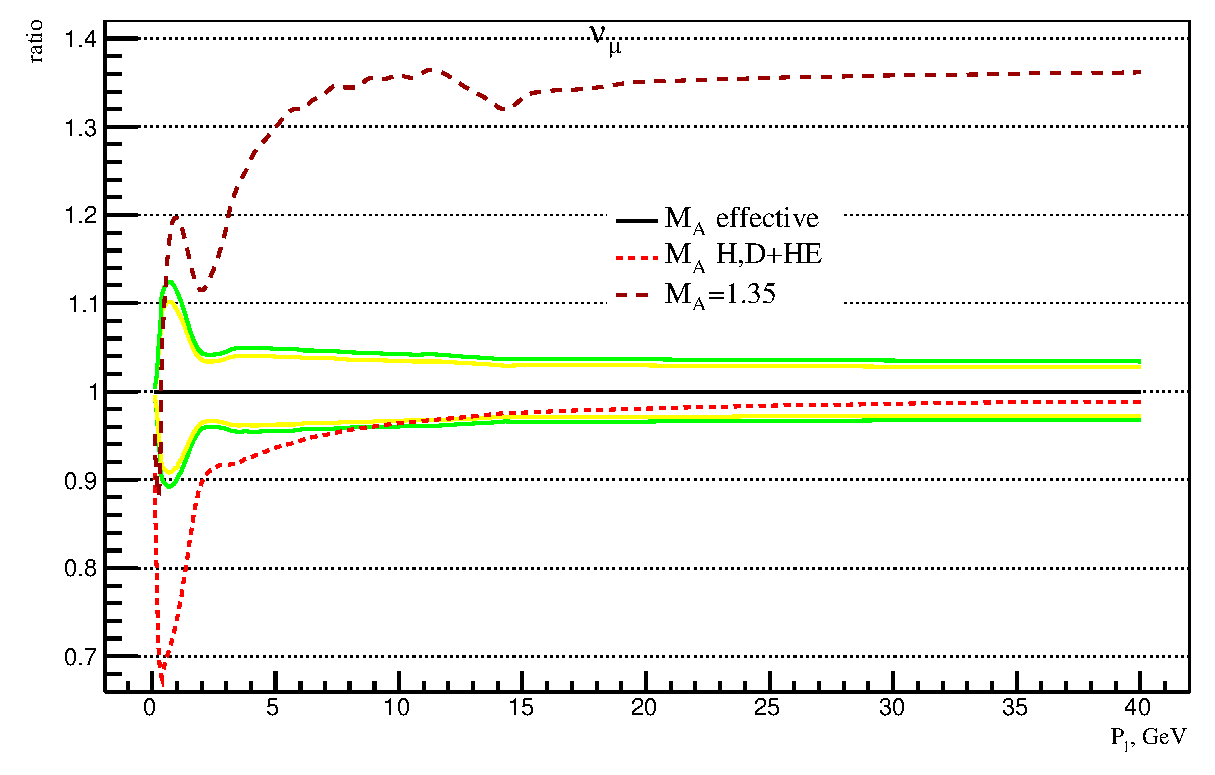
\includegraphics[width=0.9\columnwidth]{./NOvA/NOvA_newflux_Scintillator_nm_n5.eps}
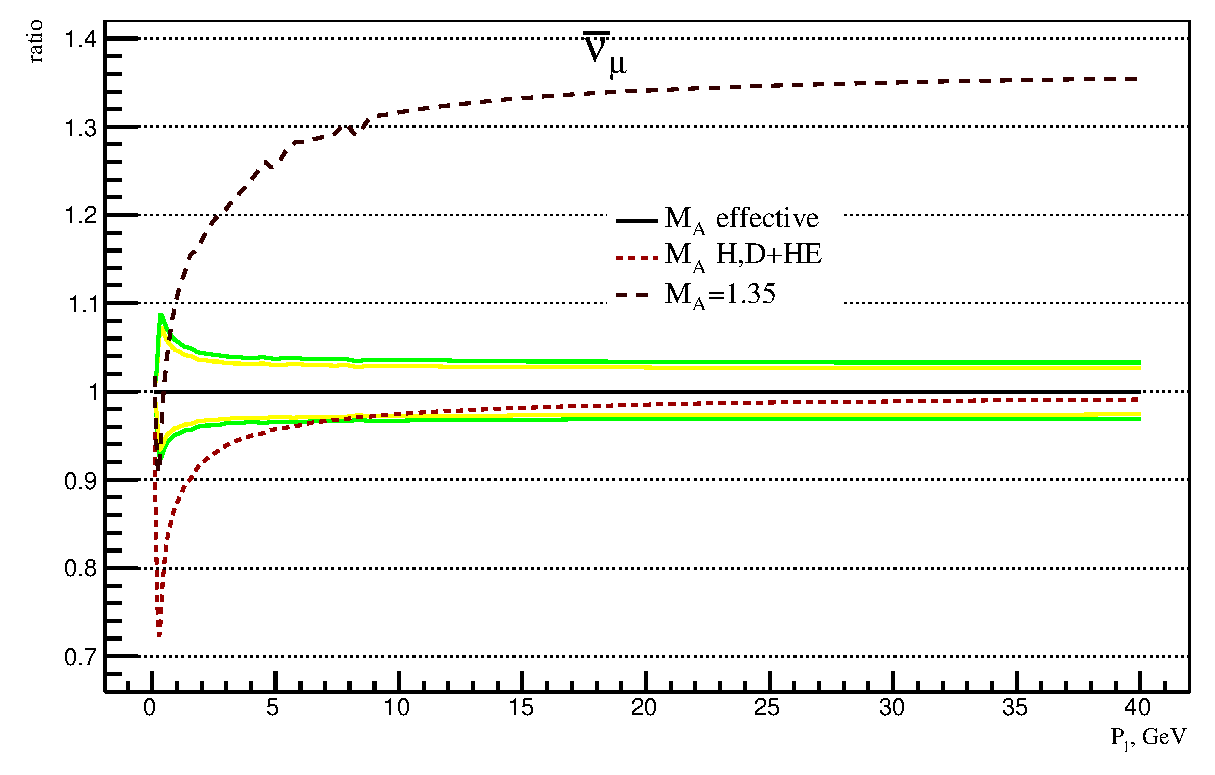
\includegraphics[width=0.9\columnwidth]{./NOvA/NOvA_newflux_Scintillator_am_n5.eps}
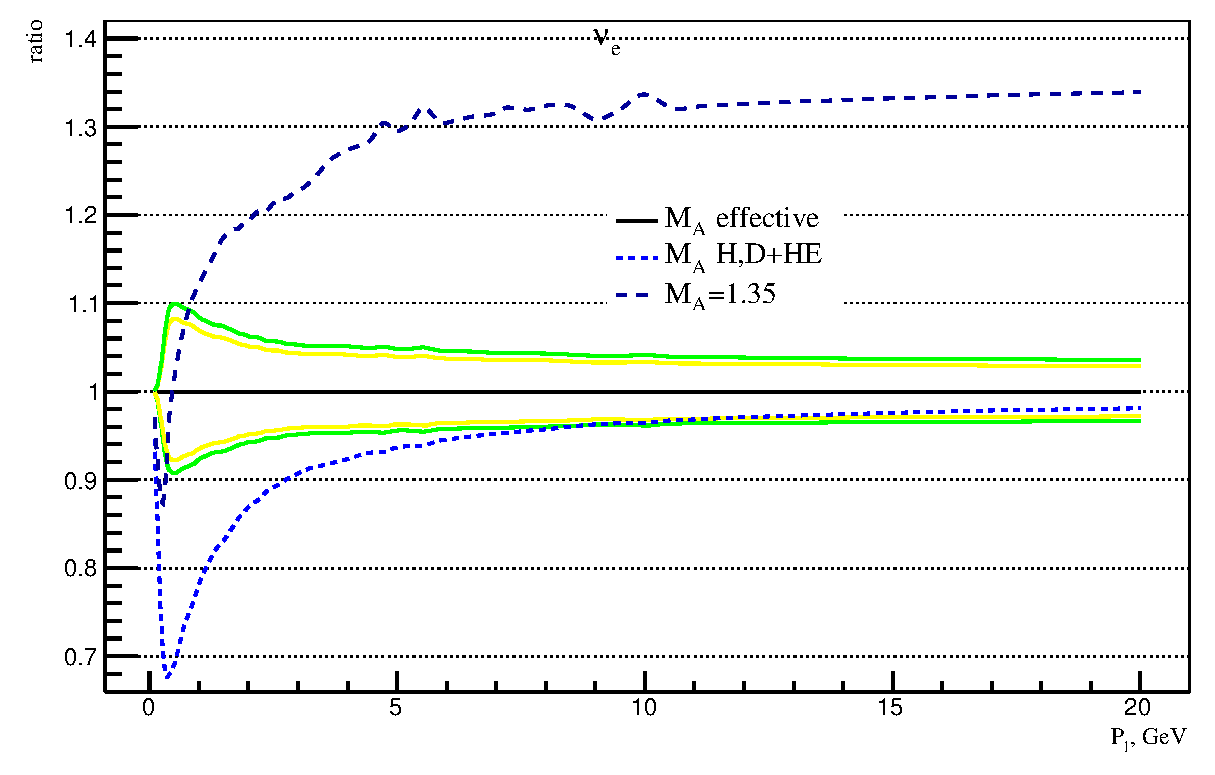
\includegraphics[width=0.9\columnwidth]{./NOvA/NOvA_newflux_Scintillator_ne_n5.eps}
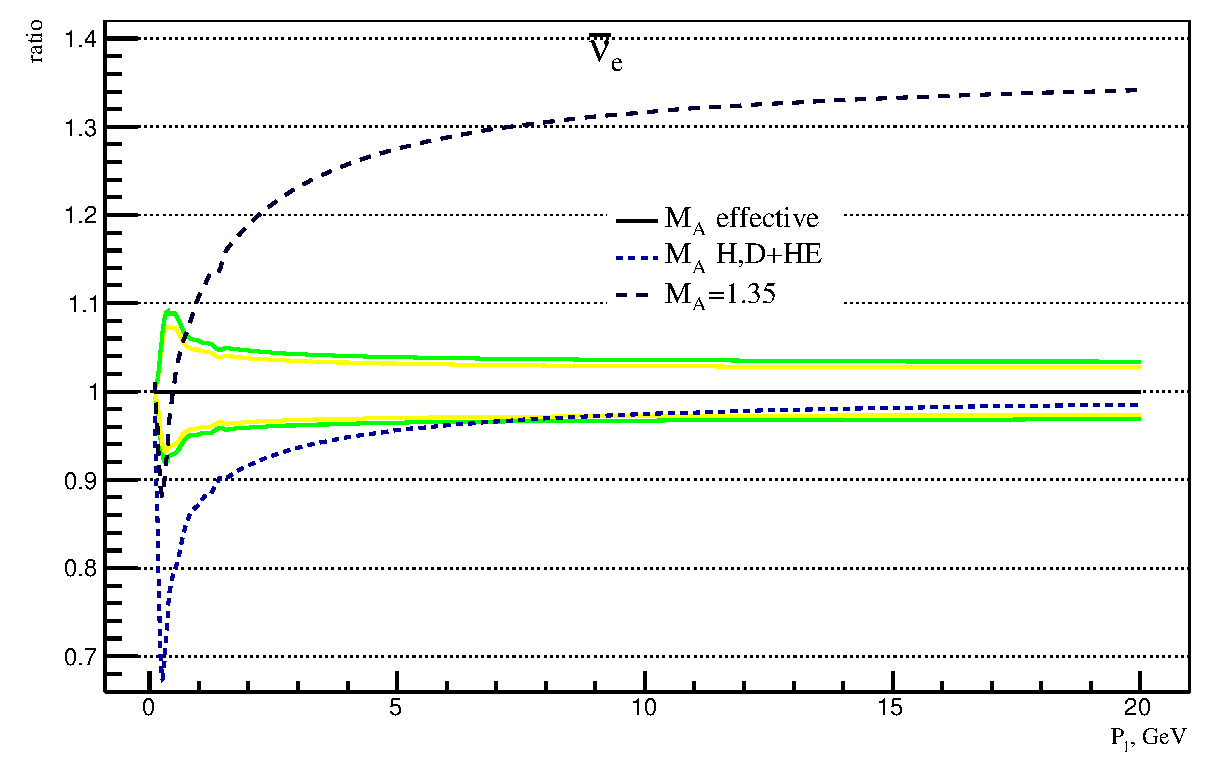
\includegraphics[width=0.9\columnwidth]{./NOvA/NOvA_newflux_Scintillator_ae_n5.eps}
\caption{\label{NOvArates}Charged lepton flux ratios in the Near Detector of NO$\nu$A experiment for $\nu$-beam mode calculated with $M_{A}$ obtained MiniBooNE experiment, deuterium best-fit $M_{A}$ value and with the effective nucleon axial mass}
\end{center}
\end{figure}

It can be seen, that the adequate choice of the axial mass value is very important to the neutrino event rate calculations: error in count rates predicted with high-energy and hydrogen/deuterium data near NO$\nu$A energy peak 2\,GeV achieves 6\%, using the MiniBooNE result $M_{A}=1.35$\,GeV~\cite{AguilarArevalo:2010zc} in high-energy region leads to approximately 30\% errors. Of course in experiments with two detectors this enormous uncertainty is roughly canceled out, but it affects experiment results through statictical uncertainties in fluxes. Because of the fact that effect depends on energy it cannot be eliminated by any renormalizing factor.

Figure~\ref{NOvAeffect} illustrates magnitude of the effect in comparison with $\nu_{\mu}\to{}\nu_{e}$ oscillation probability. Muon neutrino deficit in Far Detector, caused by oscillations to electron neutrino is comparable with deficit induced by using MiniBooNE value of $M_{A}$ at very low energies and significantly higher than one caused by exploiting best-fit deuterium $M_{A}$ value in whole energy range.

\begin{figure}[htb!]
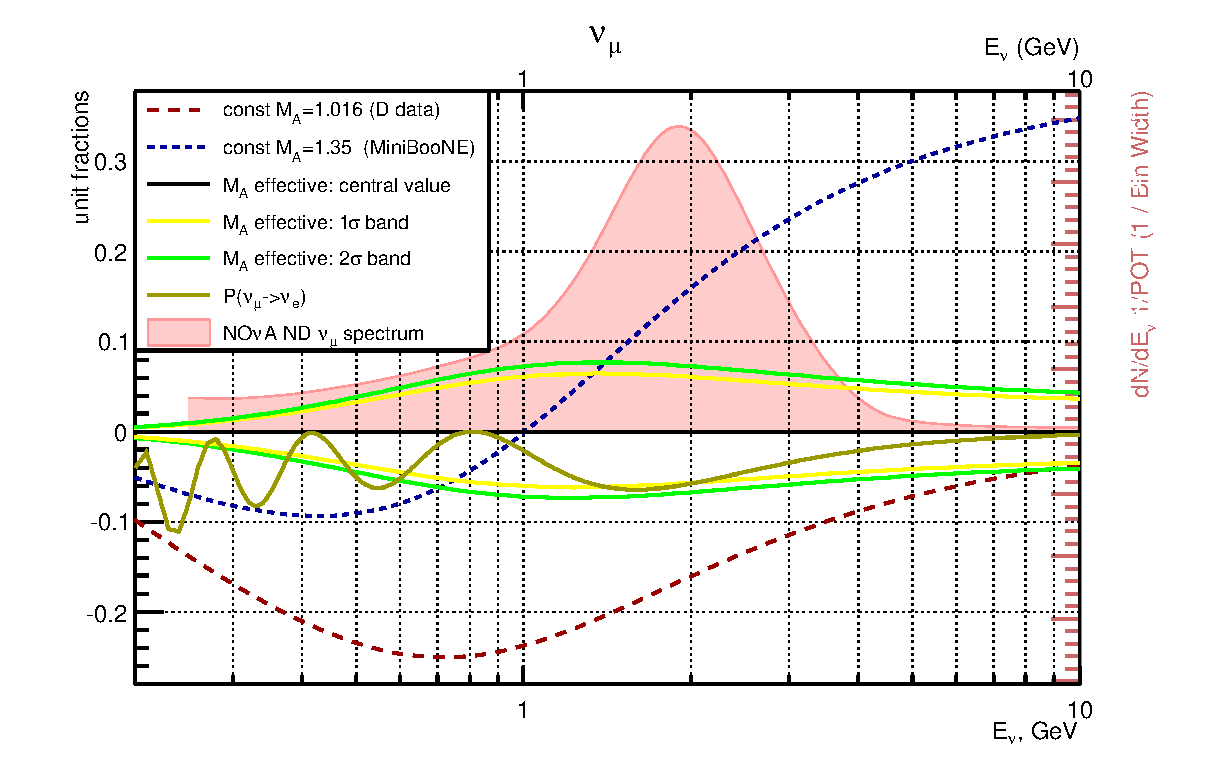
\includegraphics[width=\columnwidth]{./NOvA/Scintillator_nm_n5.eps}
\caption{\label{NOvAeffect}Comparison between $M_{A}^{\mathrm{eff}}$ impact to the total $\nu_{\mu}$ QES cross section and $P_{\nu_{\mu}\to{}\nu_{e}}$. $\nu_{\mu}$ spectrum in the Near Detector of NOvA in $\nu$-beam mode is drawn transparently in the same energy-axis for illustration}
\end{figure}

In Fig.~\ref{SKeffect} Super-Kamiokande electron-like fully-contained events mostly caused by quasielastic interactions are shown. It is seen that $M_{A}^{\mathrm{eff}}$ correction improve the agreement between MC prediction and experimental data points.

\begin{figure}[htb!]
\includegraphics[width=\columnwidth]{./SK/SK_effect_IH.eps}
\caption{\label{SKeffect}Electron-like fully-contained events in the Super-Kamiokande detector vs. lepton momentum. Blue (red) histogram corresponds to MC simulations of event rate with (without) oscillation effect. Purlpe rectangles represent blue histogram reweighed with effect of using $M_{A}^{\mathrm{eff}}$ instead of $M_{A}=1.2$\,GeV used in SK. The calculations are done for the inverse neutrino mass hierarchy}
\end{figure}

\begin{figure}[htb!]
\begin{center}
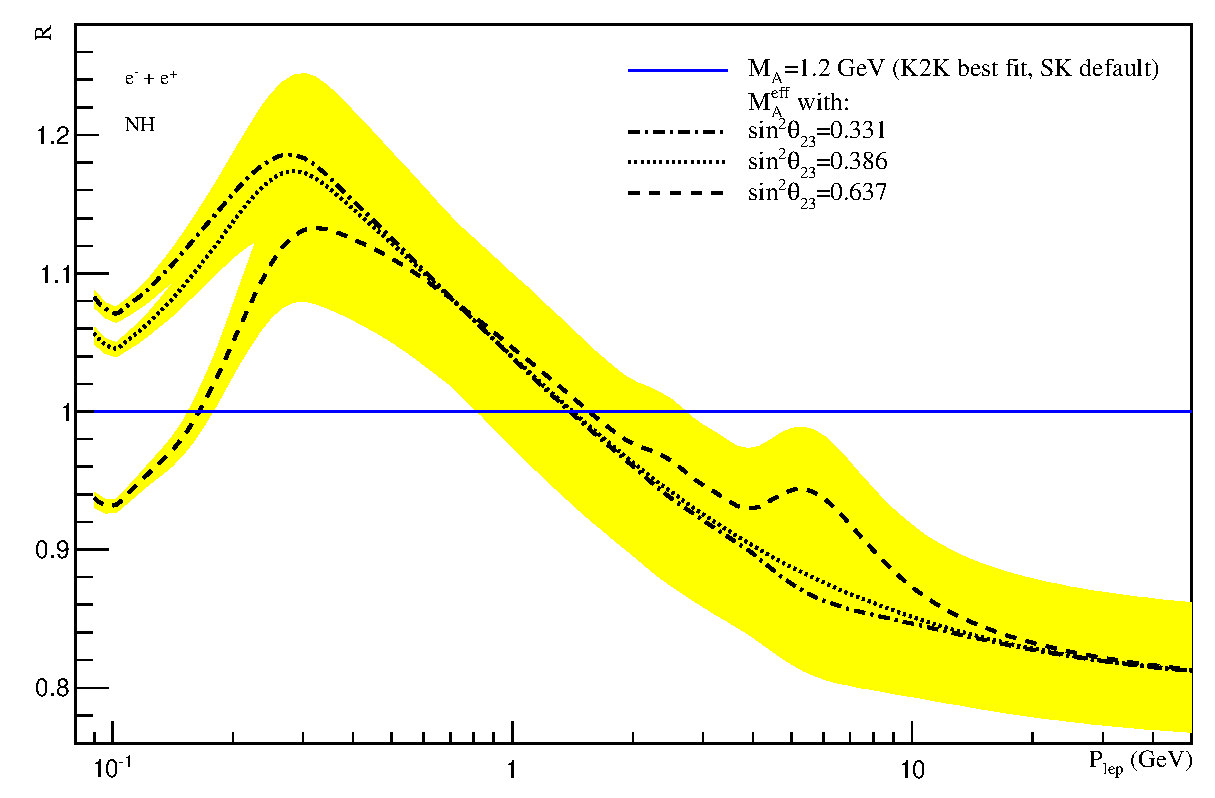
\includegraphics[width=0.9\columnwidth]{./SK/t23Ematne_11.eps}
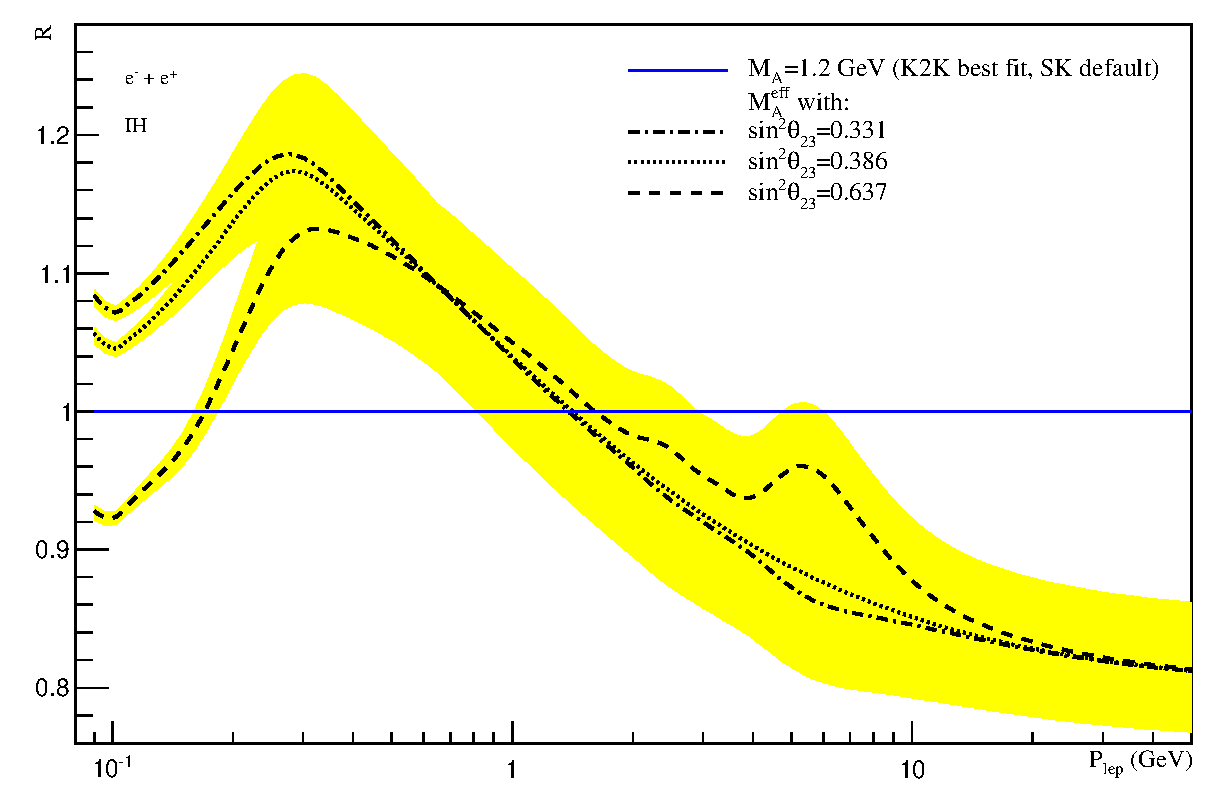
\includegraphics[width=0.9\columnwidth]{./SK/t23Ematie_11.eps}
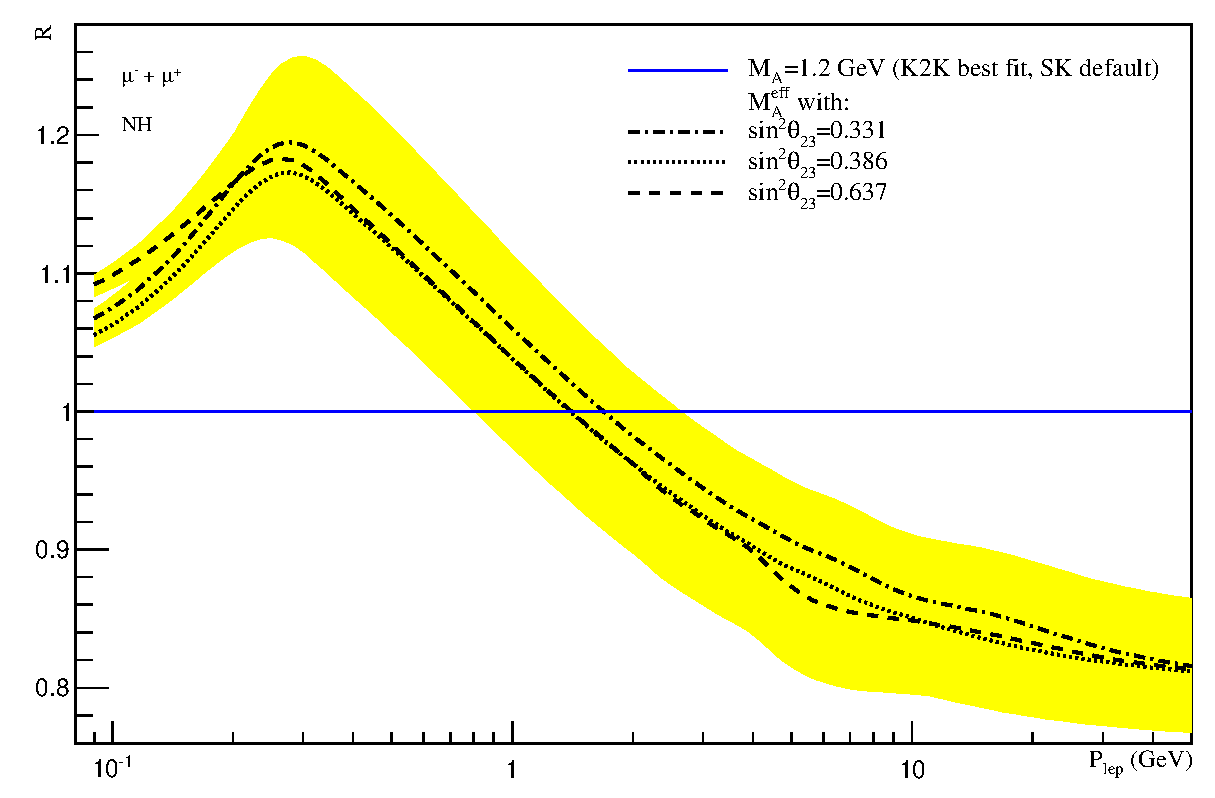
\includegraphics[width=0.9\columnwidth]{./SK/t23Ematnm_11.eps}
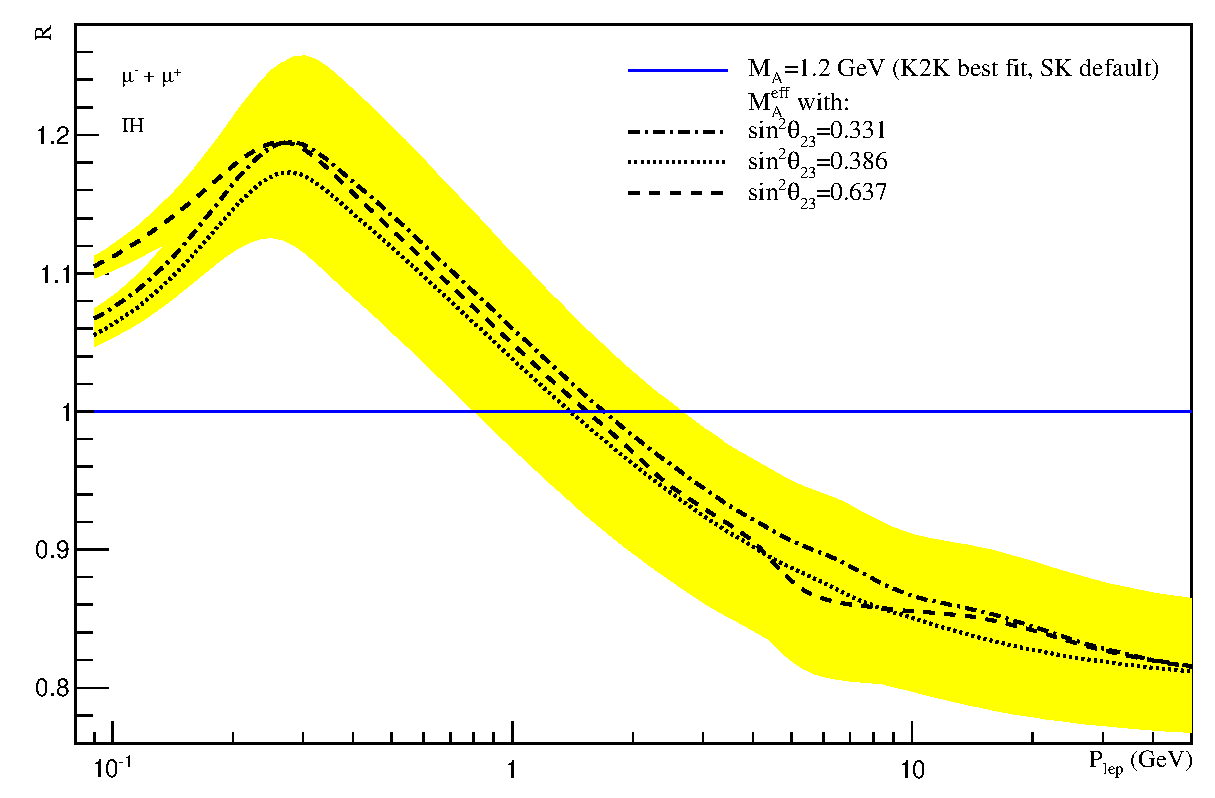
\includegraphics[width=0.9\columnwidth]{./SK/t23Ematim_11.eps}
\caption{\label{theta23}FIXME}
\end{center}
\end{figure}

\section{Conclusions}
In this paper we demonstrated that the choice of the nucleon axial mass value essentially affects the predicted count rates in the Super-Kamiokande detector particularly within the region, which the QES interactions are dominant in. The related uncertainty is comparable with that in the predicted atmospheric neutrino fluxes, as well as with the scale of the oscillation effect itself. Hence, the effect should be taken into account for the correct determination of the neutrino mixing parameters. 

Let us emphasize the fact that the estimations presented herein are preliminary. However, we believe that using the effective axial mass instead of the value 1.2\,GeV currently used by the SK Collaboration~\cite{Wendell:2010md} or the value $0.99$\,GeV used by the T2K Collaboration~\cite{Abe:2011ks} should substantially improve the validity of the extracted neutrino mixing parameter values.

Future progress in the nuclear modelling and new experiments (e.g., MINER$\nu$A) will hopefully allow us to improve the accuracy of the current $M_A$ extraction and $M_{A}^{\mathrm{eff}}$ determination.


\section*{References}
\bibliography{text/bibfile}

\end{document}
